\documentclass[sigconf]{acmart}

%% This report uses the ACM sigconf template for formatting only; it is a
%% course project report, not an ACM-sponsored publication, so the rights
%% and DOI/ISBN metadata are suppressed rather than filled with placeholders.
\settopmatter{printacmref=false, printccs=false, printfolios=true}
\setcopyright{none}
\acmConference[CSE 402]{CSE 402: Numerical Analysis, Simulation and Modeling Sessional}{2026}{Department of CSE, BUET}
\acmDOI{}
\acmISBN{}

\usepackage{array}
\newcolumntype{L}[1]{>{\raggedright\arraybackslash}p{#1}}

\begin{document}

%% -------------------------------------------------------------------------
%% TITLE, GROUP, SECTION, AUTHORS
%% -------------------------------------------------------------------------
\title{Beyond Antithetic Variates: Benchmarking Variance Reduction for Monte
Carlo Pricing of Barrier and Asian Options}

\newcommand{\groupnumber}{07}
\newcommand{\coursesection}{A}

\author{Nafis Nahian}
\affiliation{%
  \institution{Department of CSE, BUET}
  \city{Dhaka}
  \country{Bangladesh}}
\email{2105007@ugrad.cse.buet.ac.bd}

\author{Aritra Debnath}
\affiliation{%
  \institution{Department of CSE, BUET}
  \city{Dhaka}
  \country{Bangladesh}}
\email{2105010@ugrad.cse.buet.ac.bd}

\author{Tamzeed Mahfuz}
\affiliation{%
  \institution{Department of CSE, BUET}
  \city{Dhaka}
  \country{Bangladesh}}
\email{2105012@ugrad.cse.buet.ac.bd}

\author{Arnob Biswas}
\affiliation{%
  \institution{Department of CSE, BUET}
  \city{Dhaka}
  \country{Bangladesh}}
\email{2105015@ugrad.cse.buet.ac.bd}

\author{Zaki Rehnoom Unmona}
\affiliation{%
  \institution{Department of CSE, BUET}
  \city{Dhaka}
  \country{Bangladesh}}
\email{2105016@ugrad.cse.buet.ac.bd}

\renewcommand{\shortauthors}{Nahian, Debnath, Mahfuz, Biswas, and Zaki}

\begin{abstract}
The base paper prices an up-and-in barrier call and a geometric-average Asian
option by Monte Carlo under geometric Brownian motion with antithetic
variates, and names advanced variance reduction as future work. We rebuild
its experiment from scratch, validate every estimator against closed-form
prices, and reproduce its two central findings. Its antithetic speedups are
confirmed as variance ratios ($1.47\times$ barrier, $1.35\times$ Asian call)
and shown to follow from the pair correlation $\rho$ through $1/(1+\rho)$. Its
finding that the discretization scheme barely matters is confirmed and
explained: Milstein's pathwise gain (strong order $0.97$ vs.\ $0.49$) does not
reach the price, where both schemes are first order. We then add three
advanced techniques --- control variates, randomized quasi-Monte Carlo (RQMC)
with a Brownian bridge, and importance sampling --- and price the arithmetic
Asian option, which has no closed form. All five methods are benchmarked in
one interleaved run on efficiency, $1/(\text{variance}\times\text{time})$,
with bootstrap confidence intervals. At $N=65{,}536$, control variates and
RQMC are $10^2$--$10^3$ times more efficient than plain Monte Carlo on the
near-the-money barrier and both Asians; importance sampling specializes in
rare knock-ins ($\approx 49\times$ at $B=160$); antithetic variates give a
modest $1.1$--$1.5\times$. Variance reduction also exposes a $-0.011$
discrete-monitoring bias that plain Monte Carlo cannot see. We recommend RQMC
with a Brownian bridge for barrier options and the geometric-Asian control
variate for the arithmetic Asian.
\end{abstract}

\keywords{Monte Carlo simulation, variance reduction, option pricing, barrier
options, Asian options, control variates, quasi-Monte Carlo, Brownian bridge,
importance sampling}

\maketitle

\section*{Group and Section}
\noindent Group \groupnumber\ \quad Section \coursesection

\medskip
\noindent\textit{Code:} \url{https://github.com/sleepytmzd/Numerical-project-G07}

%% =========================================================================
\section{Introduction and Base Paper Review}
%% =========================================================================

\subsection{Motivation}
Monte Carlo (MC) simulation is the dominant computational tool for pricing
path-dependent exotic options, because it needs no assumption beyond the
ability to simulate the underlying stochastic process. Unlike closed-form
solutions, which exist only for special payoff structures, MC can price any
claim whose payoff is a function of the simulated path. The cost is
statistical: a crude MC estimate converges at the slow rate $O(N^{-1/2})$, so
reducing an estimator's variance without introducing bias is one of the most
practically important problems in computational finance.

\subsection{Background}
A European option gives its holder the right, not the obligation, to buy
(call) or sell (put) an asset at a fixed strike price $K$ at maturity $T$. The
Black--Scholes model~\cite{BlackScholes1973} assumes the asset follows
geometric Brownian motion (GBM) under the risk-neutral measure,
\begin{equation}
  dS_t = r S_t\,dt + \sigma S_t\,dW_t,
  \label{eq:gbm}
\end{equation}
where $S_t$ is the asset price, $r$ the risk-free rate, $\sigma$ the
volatility, and $W_t$ a standard Brownian motion. \emph{Exotic options} are
path-dependent: their payoff depends on the whole trajectory of $S_t$, not
just its terminal value.
\begin{itemize}
  \item A \textbf{barrier option} activates (``knock-in'') or extinguishes
    (``knock-out'') if the path touches a level $B$ during the option's life.
    An up-and-in call pays $(S_T-K)^+ \cdot \mathbf{1}\{\max_{0\le t\le T}
    S_t \ge B\}$. Reiner and Rubinstein~\cite{ReinerRubinstein1991} give a
    closed form under \emph{continuous} monitoring; discrete monitoring
    introduces a downward bias that Broadie, Glasserman and
    Kou~\cite{BroadieGlassermanKou1997} quantify with a continuity
    correction (``BGK'').
  \item An \textbf{Asian option} pays on the average price. The
    geometric-average Asian has a closed form~\cite{KemnaVorst1990}, because
    the geometric mean of lognormal variables is itself lognormal. The
    arithmetic-average Asian has no closed form, which is why it is the
    standard example for demonstrating that Monte Carlo is indispensable.
\end{itemize}
Exact GBM sampling at a step $\Delta t$ uses
\begin{equation}
  S_{t+\Delta t} = S_t \exp\!\big((r-\tfrac12\sigma^2)\Delta t + \sigma\sqrt{\Delta t}\,Z\big),
  \qquad Z\sim N(0,1),
  \label{eq:exact-scheme}
\end{equation}
which has zero discretization error at the grid points for any $\Delta t$.
Two alternative SDE discretizations are commonly used when no exact scheme is
available: Euler--Maruyama (strong order $0.5$) and
Milstein~\cite{KloedenPlaten1992} (strong order $1.0$, adding the It\^{o}
correction $\tfrac12\sigma^2 S_t(Z^2-1)\Delta t$). Both have \emph{weak} order
$1$, so for a price --- which is an expectation --- the scheme choice changes
the answer only at $O(\Delta t)$, far below Monte Carlo sampling error at any
practical $N$. Standard references for the following material are
Glasserman~\cite{Glasserman2004} and Boyle, Broadie and
Glasserman~\cite{BoyleBroadieGlasserman1997}. Four variance-reduction
techniques exploit different structure to beat the $O(N^{-1/2})$ wall:
\begin{enumerate}
  \item \textbf{Antithetic variates} pair each path driven by $Z$ with a
    mirror path driven by $-Z$. The pair average cancels the part of the
    payoff that is linear (odd) in $Z$ and does nothing for the even part, so
    the gain depends on how close to linear the payoff is.
  \item \textbf{Control variates} subtract a regression-adjusted residual of
    a correlated quantity with a known expectation. The optimal
    variance-reduction factor is $1/(1-\rho^2)$, where $\rho$ is the
    correlation between the target and the control.
  \item \textbf{Quasi-Monte Carlo (QMC)} replaces pseudo-random points with a
    low-discrepancy sequence (Sobol~\cite{Sobol1967,JoeKuo2008}) that fills
    the sampling space more evenly, at rates up to $O(N^{-1})$ for smooth
    integrands of low effective
    dimension~\cite{MoskowitzCaflisch1996,BoyleBroadieGlasserman1997}.
  \item \textbf{Importance sampling (IS)} simulates under a shifted measure
    so that rare but important events occur more often, then corrects with a
    likelihood ratio.
\end{enumerate}

\subsection{Base Paper Review}
\label{sec:base-paper}
The base paper~\cite{Gottimukkala2024} prices an up-and-in barrier call
($S_0=100$, $K=105$, $B=110.6772$, $\sigma=0.2$, $r=0.03$, $T=1$~year) and a
geometric-average Asian call and put, including a variant averaged over the
last 30 days, under three path-generation schemes (``Euler'',
``Euler--Maruyama'', ``Milstein''), with antithetic variates as its
variance-reduction technique, and presents its results as
confidence-interval plots against the number of paths. Where the paper leaves
implementation details open (the number of time steps, the random seed, and
the Asian strike and averaging grid), we fix them at the most plausible
values: 252 daily steps and $K=105$, the strike consistent with its figures.
Its two central findings are:
\begin{enumerate}
  \item antithetic variates accelerate convergence ``by 1.5 times for Barrier
    options and 1.3 times for Asian options'';
  \item the choice of discretization scheme has a negligible effect on
    accuracy.
\end{enumerate}
It recommends that future work prioritize ``advanced variance reduction
techniques'' over new path-generation schemes.
Section~\ref{sec:results-baseline} reproduces both findings and explains
where each comes from. The paper's scope is options with a closed form and
a single variance-reduction technique; pricing an option without a closed
form, and comparing techniques on an efficiency metric that accounts for the
extra cost each one introduces, are natural next steps that we take here.

\subsection{Our Extension}
We take up the paper's own future-work direction. Table~\ref{tab:what-we-add}
summarizes what we add on top of the base paper.

\begin{table}[t]
\caption{What the base paper did versus what we add.}
\label{tab:what-we-add}
\small
\begin{tabular}{L{0.21\linewidth}L{0.27\linewidth}L{0.33\linewidth}}
\toprule
\textbf{Aspect} & \textbf{Base paper} & \textbf{Our extension} \\
\midrule
Options & Barrier call; geometric Asian call/put, 30-day call &
  + Arithmetic Asian (no closed form); deep ($B{=}140$) and rare ($B{=}160$) barriers \\
\midrule
Variance reduction & Antithetic only &
  + Control variates, QMC with a Brownian bridge, importance sampling \\
\midrule
Antithetic gain & $\approx1.5\times$ barrier, $\approx1.3\times$ Asian &
  Reproduced ($1.47\times$, $1.35\times$); predicted by $1/(1+\rho)$ \\
\midrule
Efficiency metric & Convergence speedup &
  $1/(\text{var}\times\text{time})$ with bootstrap CI; time-to-accuracy \\
\midrule
Error metric & CI plots & RMSE against a 252-date reference price \\
\midrule
Scheme comparison & Three schemes; effect negligible &
  Reproduced; explained by measured strong order ($0.49$ / $0.97$) and weak order ($\approx1$ for both) \\
\midrule
Convergence rate & CI plots vs.\ $N$ & Plain MC $\approx N^{-1/2}$; RQMC slopes $-0.60$ to $-0.80$ \\
\midrule
Averaging window & 30-day geometric Asian & Window sensitivity quantified: $6.708$ (30 dates) vs.\ $3.000$ (full year) \\
\midrule
Barrier bias & Mentioned, not applied & Quantified ($-0.011$ paper, $-0.160$ deep, at 252 dates); BGK correction \\
\midrule
Rare events & $B=110.68$ only & $B=140$: IS $8.6\times$; $B=160$: IS $\approx 49\times$ \\
\bottomrule
\end{tabular}
\end{table}

%% =========================================================================
\section{Methodology}
%% =========================================================================

\subsection{Simulation Engine}
\label{sec:engine}
A single path-generation routine, \texttt{generate\_paths}, implements the
exact scheme (Eq.~\ref{eq:exact-scheme}) and the Euler--Maruyama and Milstein
schemes on a uniform grid of \texttt{n\_steps} steps. It never draws its own
randomness: it takes a pre-built array of standard normals of shape
$(n_{\text{paths}}, n_{\text{steps}})$ and an optional drift override. This
single frozen interface is what lets every later technique reuse the same
engine:
\begin{itemize}
  \item \textbf{Antithetic variates} build the normals array as $[Z,-Z]$.
  \item \textbf{QMC} builds the normals from a scrambled Sobol sequence via
    the inverse normal CDF, then applies the Brownian bridge as an
    orthogonal linear map before the array reaches the engine
    (Section~\ref{sec:qmc-method}).
  \item \textbf{Importance sampling} passes a shifted drift
    $\mu = r+\sigma\theta$ through the drift-override parameter, simulating
    under the tilted measure while using the \emph{same} normals and the same
    discounting; the likelihood-ratio correction is applied afterward by the
    estimator, not by the engine.
\end{itemize}
All three schemes are fully vectorized. Every estimator returns a common
record: price, standard error, 95\% confidence interval, runtime, and an
\texttt{extra} dictionary for technique-specific diagnostics (e.g.\ $\rho$ and
$\hat b$ for control variates, effective sample size for importance
sampling). A generic sweep routine loops over (scenario $\times$ scheme
$\times$ method $\times$ $N$ $\times$ replicate), logs one row per replicate,
and a shared benchmarking module aggregates rows into per-cell statistics:
mean price, variance \emph{across replicates}, bias against a reference
price, $\mathrm{RMSE}=\sqrt{\text{bias}^2+\text{variance}}$, mean runtime, and
efficiency. All randomness is seeded deterministically from one base seed, so
every run is exactly reproducible.

\subsection{Control Variates}
\label{sec:cv-method}
For a discounted target payoff $Y$, a discounted control payoff $X$ with
known expectation $\mu_X$, the control-variate estimator is
\begin{equation}
  \hat V_{\mathrm{CV}} = \frac{1}{N}\sum_{i=1}^{N}\Big[Y_i - \hat b\,(X_i-\mu_X)\Big],
  \qquad \hat b = \frac{\widehat{\mathrm{Cov}}(Y,X)}{\widehat{\mathrm{Var}}(X)}.
  \label{eq:cv}
\end{equation}
At the optimal coefficient $b^\ast=\mathrm{Cov}(Y,X)/\mathrm{Var}(X)$, the
theoretical variance-reduction factor (VRF) is
\begin{equation}
  \mathrm{VRF} = \frac{\mathrm{Var}(Y)}{\mathrm{Var}(Y-b^\ast(X-\mu_X))} = \frac{1}{1-\rho_{YX}^2}.
  \label{eq:cv-vrf}
\end{equation}
We fit $\hat b$ on an \emph{independent pilot sample} and apply it to a
separate production sample, keeping the estimator exactly unbiased. We use
the discrete geometric-average Asian as the control for the arithmetic
Asian, and the terminal European call (Black--Scholes price) as the control
for the up-and-in barrier.

\subsection{Quasi-Monte Carlo with a Brownian Bridge}
\label{sec:qmc-method}
The Koksma--Hlawka inequality bounds the QMC integration error by
$V(f)\,D^\ast(P_N)$, the variation of the integrand times the star
discrepancy of the point set, and $D^\ast(P_N)=O((\log N)^d/N)$ for a Sobol
net. In $d=252$ dimensions the bound itself is useless; fast rates appear
only when the integrand has low \emph{effective} dimension and is smooth.
A kink ($\max(\cdot,0)$) slows convergence, and a jump whose boundary is not
aligned with the coordinate axes, such as the knock-in indicator
$\mathbf 1\{\max_j S_{t_j}\ge B\}$, slows it further.

All Sobol sequences are generated with SciPy's quasi-Monte Carlo
module~\cite{Virtanen2020}. A scrambled Sobol sequence~\cite{Owen1997} is balanced only at sample sizes
that are powers of two; drawing any other $N$ silently degrades it toward
the Monte Carlo rate, so our sample grid is restricted to powers of two and
the code rejects any other $N$.
Uniform points are mapped to normals only through the inverse normal CDF,
never Box--Muller, which would mix coordinates and destroy the
low-discrepancy structure. SciPy's points are multiples of $2^{-30}$, so an
exact $0$ (with $\Phi^{-1}(0)=-\infty$) has probability $2^{-30}$ per
coordinate; each point is moved to the centre of its dyadic cell first,
which keeps every normal finite across the $\sim\!4\times10^8$ coordinates
of a sweep.

A Sobol sequence is only genuinely low-discrepancy in its first few
dimensions. Our path has 252 time steps, i.e.\ 252 dimensions, so assigning
dimension $j$ to time step $j$ (the ``incremental'' construction) wastes most
of the sequence's advantage on high-index dimensions where it is no better
than random. The \textbf{Brownian bridge}~\cite{CaflischMorokoffOwen1997}
instead builds the path outside-in: dimension 0 sets the terminal value
$W_T$, dimension 1 sets the midpoint $W_{T/2}$ conditional on $W_T$, and
later dimensions fill in successive midpoints by recursive bisection,
\begin{equation}
  W_t \mid W_{t_l}, W_{t_r} \sim \mathcal N\!\Big(
    \tfrac{(t_r-t)W_{t_l}+(t-t_l)W_{t_r}}{t_r-t_l},\;
    \tfrac{(t-t_l)(t_r-t)}{t_r-t_l}\Big),
  \qquad t_l<t<t_r.
  \label{eq:bridge}
\end{equation}
This is an orthogonal linear map of the input normals, so the law of the
simulated path is unchanged; only which input dimension drives which
feature of the path changes. Randomized QMC (RQMC) draws $R$ independent
scrambles of the same Sobol net; this is the \emph{only} valid source of
error bars for QMC, since the points within one scramble are not
independent. Each scramble is unbiased, so our RQMC estimator returns one
price per scramble and logs its within-run standard error and confidence
interval as NaN by design; every RQMC error bar in this paper comes from the
spread across the $R$ scrambles.

\subsection{Discretization Order}
\label{sec:scheme-method}
For $dS_t=rS_t\,dt+\sigma S_t\,dW_t$ with step $\Delta t$ and
$Z_j\sim N(0,1)$, the two discretizations are
\begin{align}
  S_{j+1}^{\mathrm{EM}} &= S_j\big(1+r\Delta t+\sigma\sqrt{\Delta t}\,Z_j\big),
  \label{eq:em}\\
  S_{j+1}^{\mathrm{Mil}} &= S_j\big(1+r\Delta t+\sigma\sqrt{\Delta t}\,Z_j
    + \tfrac12\sigma^2\Delta t\,(Z_j^2-1)\big),
  \label{eq:milstein}
\end{align}
against the exact step of Eq.~\ref{eq:exact-scheme}, which uses the same
$Z_j$. We measure the \emph{strong} (pathwise) error
$E|S_T^{\Delta t}-S_T|$ and the \emph{weak} (price) error
$|E[f(S^{\Delta t})]-E[f(S)]|$ for a payoff $f$, and fit their orders as
log--log slopes against $\Delta t$. Theory gives strong order $0.5$
(Euler--Maruyama) and $1.0$ (Milstein), and weak order $1$ for both. A price
is an expectation, so it depends only on the weak order. Both step factors
have mean $1+r\Delta t$, which gives the exact identity
$E[S_T^{\Delta t}]-E[S_T]=S_0(1+r\Delta t)^m-S_0e^{rT}$ ($m=T/\Delta t$), an
analytic check on the simulation.

\subsection{Importance Sampling}
\label{sec:is-method}
Importance sampling simulates under a shifted drift $\mu=r+\sigma\theta$ and
corrects with a likelihood ratio. Writing $\tilde W$ for the Brownian motion
built from the simulated normals, the risk-neutral Brownian motion is
$W=\tilde W+\theta t$, and by Girsanov's theorem the likelihood ratio
telescopes to a function of the terminal value alone:
\begin{equation}
  L = \exp\!\Big(-\theta \tilde W_T - \tfrac12\theta^2 T\Big).
  \label{eq:is-lr}
\end{equation}
The estimator is the sample mean of $L\cdot Y$, unbiased for any fixed
$\theta$. The drift is chosen by a heuristic that places the expected
terminal log-price on the barrier,
\begin{equation}
  \theta_0 = \frac{1}{\sigma}\Big[\frac{\ln(B/S_0)}{T} - \big(r-\tfrac12\sigma^2\big)\Big],
  \label{eq:theta0}
\end{equation}
followed by a 7-point pilot search over $\theta_0\cdot\{0,0.25,\dots,1.5\}$ on
an independent 10{,}000-path pilot, minimizing the empirical second moment of
the weighted payoff. Every estimate reports the Kish effective sample
size~\cite{Kish1965}, $\mathrm{ESS}=(\sum_i w_i)^2/\sum_i w_i^2$, and the
maximum weight, which
together diagnose whether the result rests on a handful of paths.

\subsection{Benchmarking and Acceptance Criteria}
\label{sec:acceptance}
Every estimator is validated against four criteria fixed before any
experiment was run: (1)~within 3 standard errors of a reference price
wherever one exists; (2)~95\% confidence-interval coverage across replicates;
(3)~every speedup reported as efficiency $=1/(\text{variance}\times
\text{time})$ with a bootstrap confidence interval~\cite{EfronTibshirani1993}
(2{,}000 resamples), since
with $R=20$ replicates a variance estimate alone carries about $\pm32\%$
relative error; and (4)~error reported as RMSE, not variance alone, since a
biased low-variance estimator would otherwise look artificially good. RQMC
has no valid within-run standard error, so its coverage is instead checked
with a $t$-interval over its $R$ independent scrambles.

%% =========================================================================
\section{Implementation and Experiments}
%% =========================================================================

\subsection{Scenarios and Protocol}
All scenarios share $S_0{=}100$, $r{=}0.03$, $\sigma{=}0.2$, $T{=}1$~year,
$K{=}105$, 252 daily monitoring dates, sample grid $N\in\{256, 1024, 4096,
16384, 65536\}$ (powers of two, for QMC), and $R=20$ independent replications
per cell, all seeded from one deterministic base seed
(Table~\ref{tab:scenarios}).

\begin{table}[t]
\caption{Frozen scenarios used throughout the experiments.}
\label{tab:scenarios}
\small
\begin{tabular}{llc}
\toprule
\textbf{Scenario} & \textbf{Type} & \textbf{Barrier $B$} \\
\midrule
\texttt{paper\_barrier} & Up-and-in call & 110.6772 \\
\texttt{mid\_barrier} & Up-and-in call (parity check) & 130 \\
\texttt{deep\_barrier} & Up-and-in call & 140 \\
\texttt{rare\_barrier} & Up-and-in call (extension) & 160 \\
\texttt{paper\_asian\_geo} & Geometric Asian call/put & --- \\
\texttt{asian\_30d} & Geometric Asian, last 30 days & --- \\
\texttt{asian\_arith} & Arithmetic Asian call (no closed form) & --- \\
\bottomrule
\end{tabular}
\end{table}

\subsection{Reference Prices}
\label{sec:refs}
The Asian references are closed forms. For the barriers, the continuous
Reiner--Rubinstein formula would conflate the discrete-monitoring bias with
sampling error once a variance-reduced estimator's error drops low enough, so
every barrier RMSE is instead measured against a dedicated 252-date reference
built from 64 independent bridge scrambles at $N=65{,}536$, on a seed stream
separate from every sweep (Table~\ref{tab:refs}). The paper-barrier reference
agrees with the in-out-parity value of the baseline replication
($7.0941\pm0.0002$, $0.15$ combined SE) and with the control-variate value
($7.093583$, $1.86$ combined SE). The arithmetic Asian's reference
($3.162981\pm0.000064$) is built the same way.

\begin{table}[t]
\caption{252-date (daily-monitoring) reference prices used for every barrier
RMSE, against the continuous Reiner--Rubinstein and BGK values.}
\label{tab:refs}
\small
\begin{tabular}{lccc}
\toprule
\textbf{Barrier} & \textbf{252-date reference} & \textbf{Continuous} & \textbf{BGK} \\
\midrule
$B=110.68$ & $7.094133\pm0.000096$ & $7.105528$ & $7.092995$ \\
$B=140$ & $3.385730\pm0.001014$ & $3.545321$ & $3.377810$ \\
\bottomrule
\end{tabular}
\end{table}

\subsection{Baseline Replication}
We first reproduce the base paper's own setup: the barrier call under all
three discretization schemes (paired by sharing random numbers across
schemes), and the geometric Asian call, put, and 30-day-window call under the
exact scheme, each with plain MC and antithetic variates. Two
high-precision reference runs validate the sampling: a 4{,}000{,}000-path
in-out-parity computation of the 252-date barrier price, and a
1{,}000{,}000-path common-random-number comparison of the three
discretization schemes against the exact scheme.

\subsection{Discretization-Order Experiment}
\label{sec:scheme-exp}
To explain the base paper's scheme finding, a dedicated experiment measures
the strong and weak order of Euler--Maruyama and Milstein directly (Section~\ref{sec:scheme-method}) for
$\Delta t=1/4,\ldots,1/512$, using one shared 512-step Brownian path per
sample (coarsened to each step size) so every scheme and step size sees the
same underlying randomness. Errors are taken against the exact scheme on the
same grid, which isolates the scheme error from the barrier's monitoring
bias ($20\times65{,}536$ paths per step size).

\subsection{Control Variates and the Arithmetic Asian}
The arithmetic-average payoff is the mean of the 252 simulated monitoring
prices, run at every $N$ in the grid with $R=20$ replications, using the
discrete geometric Asian as the control (Section~\ref{sec:cv-method}). Since
the arithmetic Asian has no closed form, an independent
2{,}000{,}000-path plain-MC run provides an external validation value. The
same control-variate machinery, with the terminal European call as control,
is applied to the paper barrier and to a deep barrier ($B=140$) to contrast a
near-perfect control with a weak one. A separate sweep at 12, 52, and 252
monitoring dates, with the Broadie--Glasserman--Kou continuity
correction~\cite{BroadieGlassermanKou1997} applied for comparison, isolates
the discrete-monitoring bias.

\subsection{Quasi-Monte Carlo Experiments}
Before pricing any option, the RQMC implementation is validated on two
integrals with known closed-form answers: a smooth 8-dimensional exponential
integral and a discontinuous 2-dimensional Gaussian orthant probability
(32 scrambles, $N=2^6\ldots2^{14}$). RQMC's RMSE slopes are $-0.83$ and
$-0.77$, against $-0.43$ and $-0.50$ for plain MC, with RMSE ratios of
$29\times$ and $18\times$ at $N=16{,}384$. The main sweep compares
plain MC, bridge-constructed RQMC, and incremental-constructed RQMC on the
geometric Asian call and on the paper and deep barriers ($R=20$ scrambles
per cell), with barrier RMSE measured against the 252-date references of
Section~\ref{sec:refs}.

\subsection{Importance Sampling Experiments}
Before any option is priced, the likelihood-ratio machinery is validated by
estimating a known tail probability, $P(Z>4)$, under a shifted proposal, and
checking it against the exact value. The main sweep compares plain MC,
antithetic variates, and importance sampling on the paper barrier, the deep
barrier, and a runtime-only extension scenario, \texttt{rare\_barrier}
($B=160$), added because the deep barrier's 9.3\% knock-in rate turned out
not to be genuinely rare. A fixed-$\theta$ scan over $\theta_0\cdot[0,3]$ with
common random numbers across $\theta$ traces the full per-path-variance
curve that the 7-point pilot search samples from.

\subsection{Master Comparison}
\label{sec:master-protocol}
A final experiment benchmarks all five methods together, on one machine,
single-threaded, so that the timings behind the efficiency metric are
directly comparable. The sweep covers 17 (scenario, method) cells $\times$
the $N$ grid $\times$ $R=20$: both barriers with all five methods; the
arithmetic Asian with plain, antithetic, control variate, and RQMC; and the
geometric Asian with plain, antithetic, and RQMC (the control variate is not
applicable to an option that already has a closed form, and importance
sampling targets barrier crossings specifically). Every runtime includes all
of a method's own overhead: control-variate and importance-sampling pilot
runs, and RQMC's Sobol scramble. An initial attempt ran each method as one
uninterrupted block and found machine-speed drift in its first two minutes
inflating one scenario's timings relative to another's by up to $2\times$ for
identical work; the final sweep instead \emph{interleaves} all 17 cells in a
freshly shuffled order within each (replicate, $N$) block, after an untimed
warm-up pass. All 1{,}700 prices from the interleaved run are bit-identical
to the blocked run, confirming that only the timing changed.

%% =========================================================================
\section{Results and Discussion}
%% =========================================================================

\subsection{Baseline Validation and Reproduction of the Base Paper's Findings}
\label{sec:results-baseline}
Every baseline estimator lands within 3 standard errors of its closed-form
reference in 98--100\% of replicates, and 95\% confidence-interval coverage,
pooled over all five $N$, is 91--98\%, meeting both acceptance criteria from
Section~\ref{sec:acceptance}. Figure~\ref{fig:baseline-barrier} shows the
estimated price and confidence interval against $N$ for the barrier call.
Table~\ref{tab:paper-claims} summarizes our reproduction of the base paper's
two central findings (Section~\ref{sec:base-paper}); both hold, and the rest
of this subsection explains why.

\begin{figure*}[t]
  \centering
  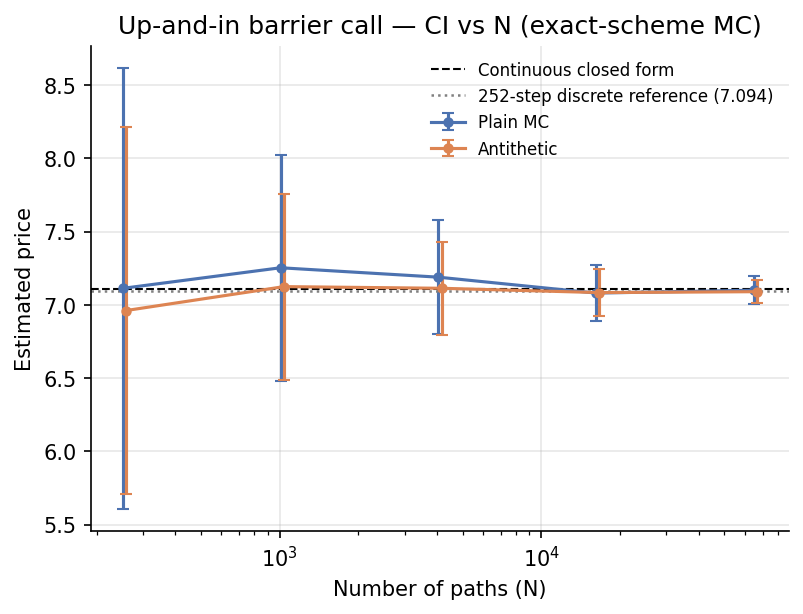
\includegraphics[width=0.85\linewidth]{figures/baseline_barrier_ci.png}
  \caption{Baseline replication: estimated price $\pm$ 95\% CI vs.\ $N$ for
  the up-and-in barrier call, plain MC and antithetic variates, against the
  continuous closed form (dashed) and the 252-date reference (dotted).}
  \label{fig:baseline-barrier}
  \Description{A convergence plot showing estimated price with confidence
  intervals shrinking as the number of simulated paths increases, straddling
  the true reference price at every sample size.}
\end{figure*}

\begin{table}[t]
\caption{Reproduction of the base paper's two central findings.}
\label{tab:paper-claims}
\small
\begin{tabular}{L{0.28\linewidth}L{0.58\linewidth}}
\toprule
\textbf{Base-paper finding} & \textbf{Our reproduction} \\
\midrule
Antithetic variates accelerate convergence $\approx1.5\times$ (barrier),
$\approx1.3\times$ (Asian) &
  \textbf{Reproduced.} Variance ratio at equal path count $1.47\times$
  (barrier) and $1.35\times$ (Asian call), stable across the whole $N$ grid
  ($1.44$--$1.48$; $1.34$--$1.53$); predicted by $1/(1+\rho)$ \\
\addlinespace
Discretization scheme has a negligible effect &
  \textbf{Reproduced.} Price difference from the exact scheme
  $-0.00057$ (Euler--Maruyama) and $-0.00105$ (Milstein) at daily steps,
  about $50\times$ below the plain-MC standard error at $N=65{,}536$;
  explained by weak order $1$ for both schemes \\
\bottomrule
\end{tabular}
\end{table}

\paragraph{Why the antithetic gain is $1.5\times$ and $1.3\times$} With $N$
paths arranged as $N/2$ antithetic pairs, the estimator's variance is
$\sigma_Y^2(1+\rho)/N$, where $\rho=\mathrm{Corr}(Y,Y')$ is the correlation
between a path's discounted payoff and its mirror's, so the variance ratio
against plain MC at equal path count is exactly $1/(1+\rho)$. The measured
pair correlations predict the measured ratios to within the rounding of $\rho$:
$\rho=-0.32\Rightarrow1.47\times$ (barrier), $\rho=-0.26\Rightarrow1.35\times$
(geometric Asian call), and $\rho=-0.32\Rightarrow1.48\times$ for the
30-day-window call. The same relation explains the Asian \emph{put}: at
$K=105>S_0$ the put is usually in the money, so its payoff is close to
linear (odd) in the driving normals, the pair correlation reaches
$\rho=-0.74$, and the gain rises to $3.91\times$. The relation also predicts
where antithetic variates help less. As the payoff becomes less linear in
$Z$, $\rho$ moves toward $0$: the within-run ratio falls from $1.5\times$ on
the paper barrier to $1.1\times$ on the deep barrier ($B=140$) and
$\approx1.0\times$ on the rare barrier ($B=160$), and it is $1.4\times$ on
the arithmetic Asian. In the single-machine master sweep
(Section~\ref{sec:results-master}) antithetic costs about the same per path
as plain MC on the paper barrier and the Asians (time ratio $0.94$--$0.99$; $0.73$ on the deep barrier), so there its efficiency gain is essentially its variance ratio. These ratios are measured within each run
from $N/2$ independent pairs; the across-replicate ratio at $R=20$ has a
sampling range of roughly $[0.4,2.5]\times$, too wide to distinguish $1.3$
from $1.5$, which is why we report the within-run value.

\paragraph{Why the scheme choice is negligible} Measured directly with common
random numbers (Section~\ref{sec:scheme-exp}), Euler--Maruyama has strong
order $0.49$ and Milstein $0.97$, matching theory
(Figure~\ref{fig:scheme-strong}). For a price, however, only the weak order
matters, and both schemes have weak order $\approx1$ on both the vanilla
call and the barrier (Figure~\ref{fig:scheme-weak}): $1.01$/$0.99$ on the
call and $1.03$/$0.99$ on the barrier (Euler--Maruyama/Milstein). The
simulated $E[S_T]$ error matches the exact identity of
Section~\ref{sec:scheme-method} within 3 SE at all eight step sizes. At
$\Delta t=1/256$, Milstein's pathwise error is $66\times$ smaller than
Euler--Maruyama's ($0.0022$ vs.\ $0.145$), yet the two barrier price biases
are of the same size ($-0.00104$ and $-0.00078$), and both are $47\times$
smaller than the plain-MC standard error at $N=65{,}536$ and $171\times$
smaller at $N=5{,}000$. At any practical sample size, then, the three
schemes produce visually indistinguishable price estimates
(Figure~\ref{fig:scheme-baseline}), exactly as the base paper reports; our
order study shows that this is a consequence of weak-order theory and will
carry over to other payoffs under GBM at daily steps. A practical corollary is that
under GBM the exact log-normal step, which has \emph{zero} discretization
error, costs about the same as either scheme ($0.64$\,s, against $0.54$\,s
for Euler--Maruyama and $0.77$\,s for Milstein per $65{,}536$ paths at
$m=512$), so we use it for every later experiment.

\begin{figure}[t]
  \centering
  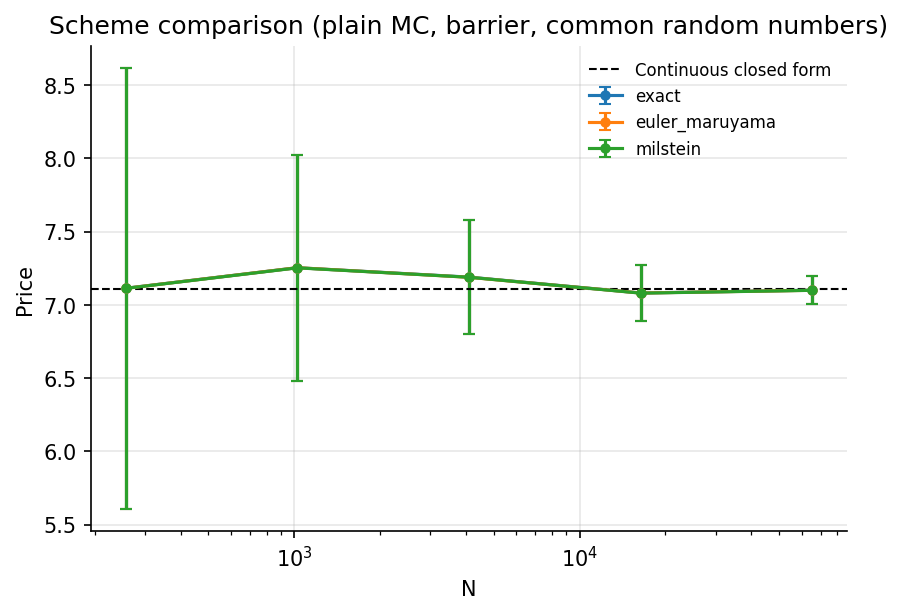
\includegraphics[width=\linewidth]{figures/baseline_scheme_comparison.png}
  \caption{Barrier price $\pm$ 95\% CI vs.\ $N$ under the exact,
  Euler--Maruyama, and Milstein schemes with common random numbers: the
  three curves coincide at every $N$.}
  \label{fig:scheme-baseline}
  \Description{A convergence plot of the barrier option price for three
  discretization schemes; the three lines and their confidence intervals lie
  exactly on top of each other at every sample size.}
\end{figure}

\begin{figure}[t]
  \centering
  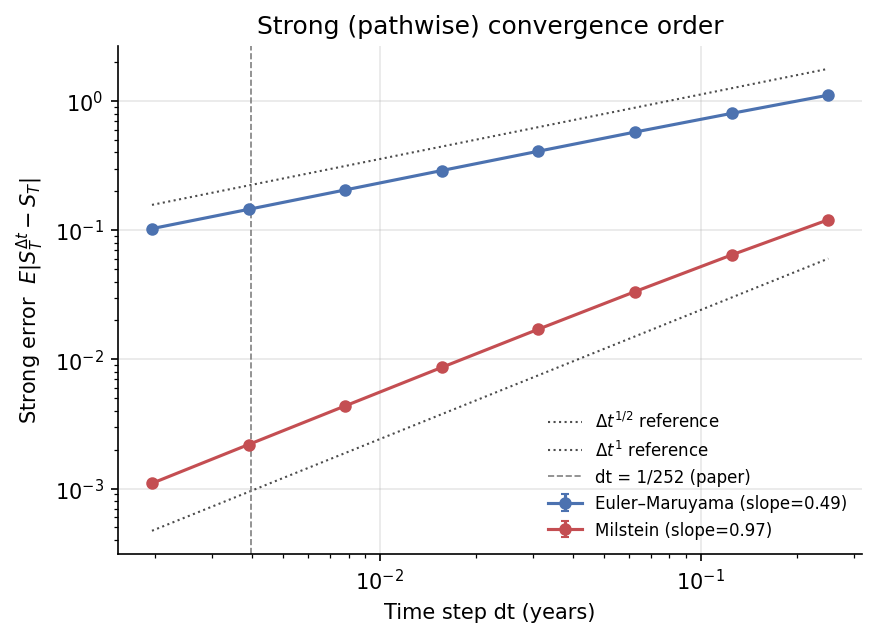
\includegraphics[width=\linewidth]{figures/scheme_strong_order.png}
  \caption{Strong-order convergence of Euler--Maruyama and Milstein: fitted
  slopes $0.49$ and $0.97$, matching the theoretical $0.5$ and $1.0$.}
  \label{fig:scheme-strong}
  \Description{A log-log plot of pathwise discretization error against step
  size for two numerical schemes, with the more refined scheme's error
  falling much faster.}
\end{figure}

\begin{figure}[t]
  \centering
  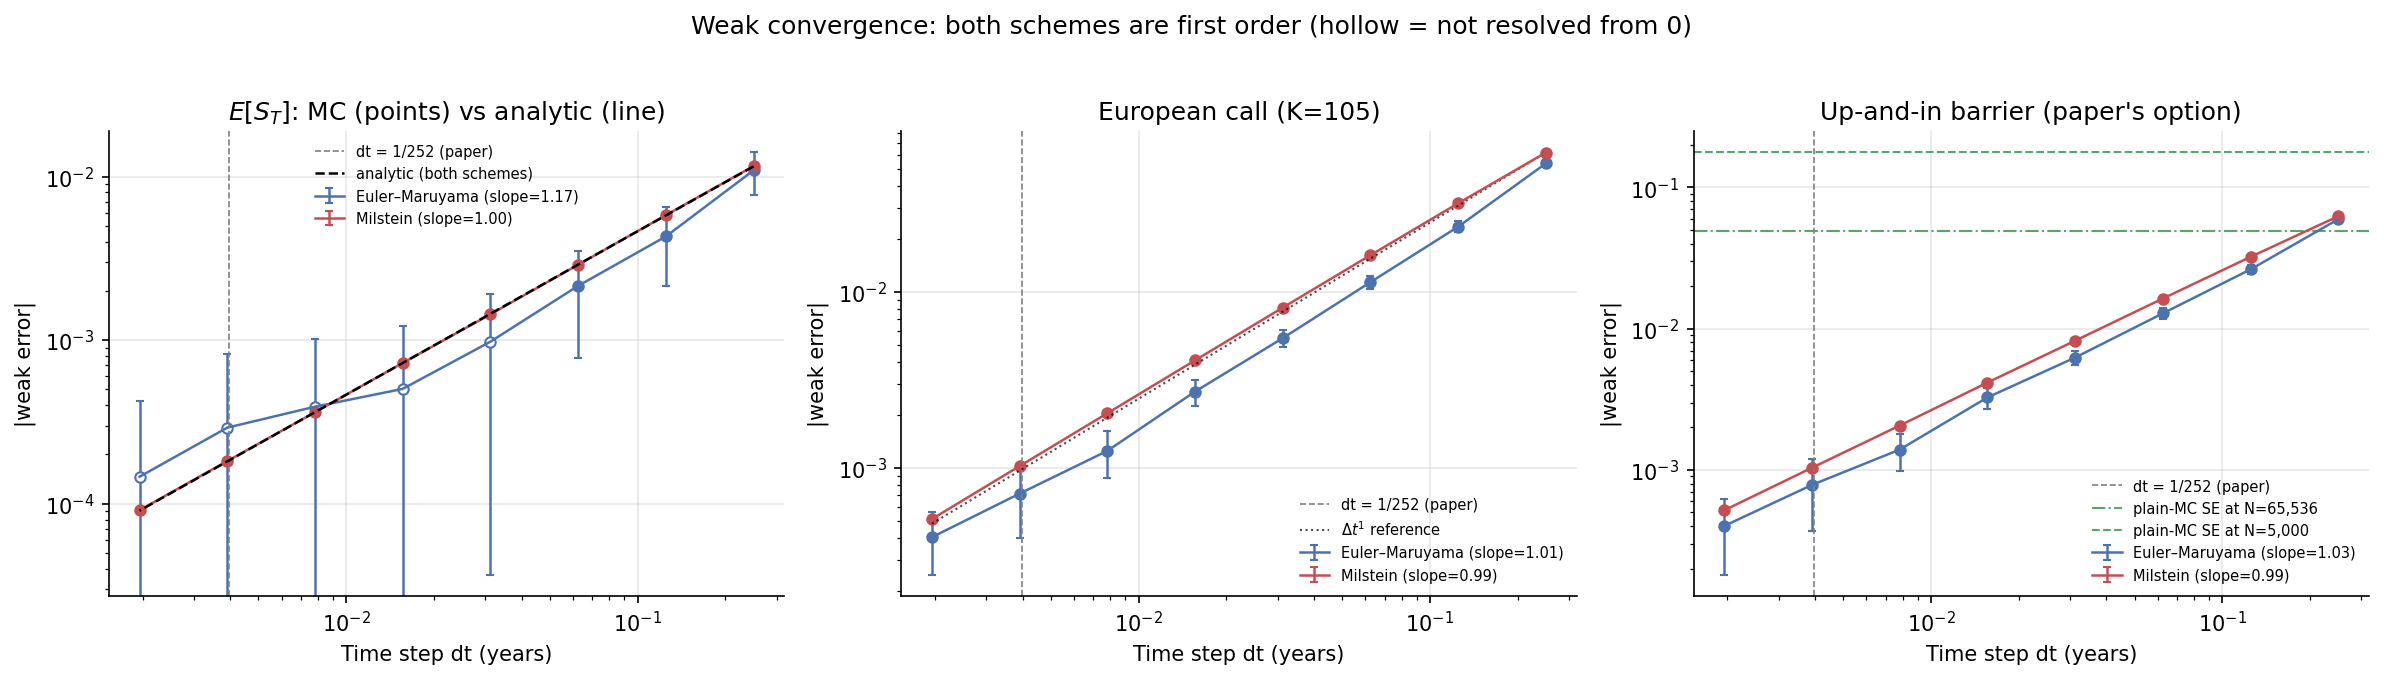
\includegraphics[width=\linewidth]{figures/scheme_weak_order.png}
  \caption{Weak-order convergence of both schemes for the terminal price and
  the barrier option: both close to the theoretical order 1, and
  indistinguishable from each other at practical sample sizes.}
  \label{fig:scheme-weak}
  \Description{A log-log plot of pricing error against step size for two
  numerical schemes, with both lines nearly overlapping, showing that the
  schemes are equally accurate for pricing.}
\end{figure}

\subsection{Additional Baseline Findings}
\label{sec:results-baseline-extra}
\paragraph{Convergence rate and the cost of precision} Across all eight
baseline scenario/method pairs, RMSE falls with fitted slopes of $-0.45$ to
$-0.52$, consistent with the theoretical $N^{-1/2}$
(Figure~\ref{fig:baseline-rmse}), and $\mathrm{RMSE}\cdot\sqrt N$ stays
roughly constant over the grid ($9.5$--$14.3$ for the barrier, $3.9$--$6.8$
for the Asian call): the error keeps shrinking at the same rate, with no
threshold beyond which extra paths stop helping. The practical consequence
is the cost of precision. With per-path standard deviations of $12.55$
(barrier) and $5.86$ (Asian call), the 95\% confidence interval is still
$\pm4.9\%$ of the barrier price at $N=5{,}000$ and $\pm12\%$ of the Asian
price at $N=1{,}000$, and reaching $\pm1\%$ needs about $1.2\times10^5$ and
$1.5\times10^5$ paths respectively. Confidence-interval plots on a
logarithmic $N$ axis look settled after a few thousand paths, but each
further halving of the error still costs four times the work; this is the
wall that the variance-reduction techniques of the following sections
attack.

\begin{figure*}[t]
  \centering
  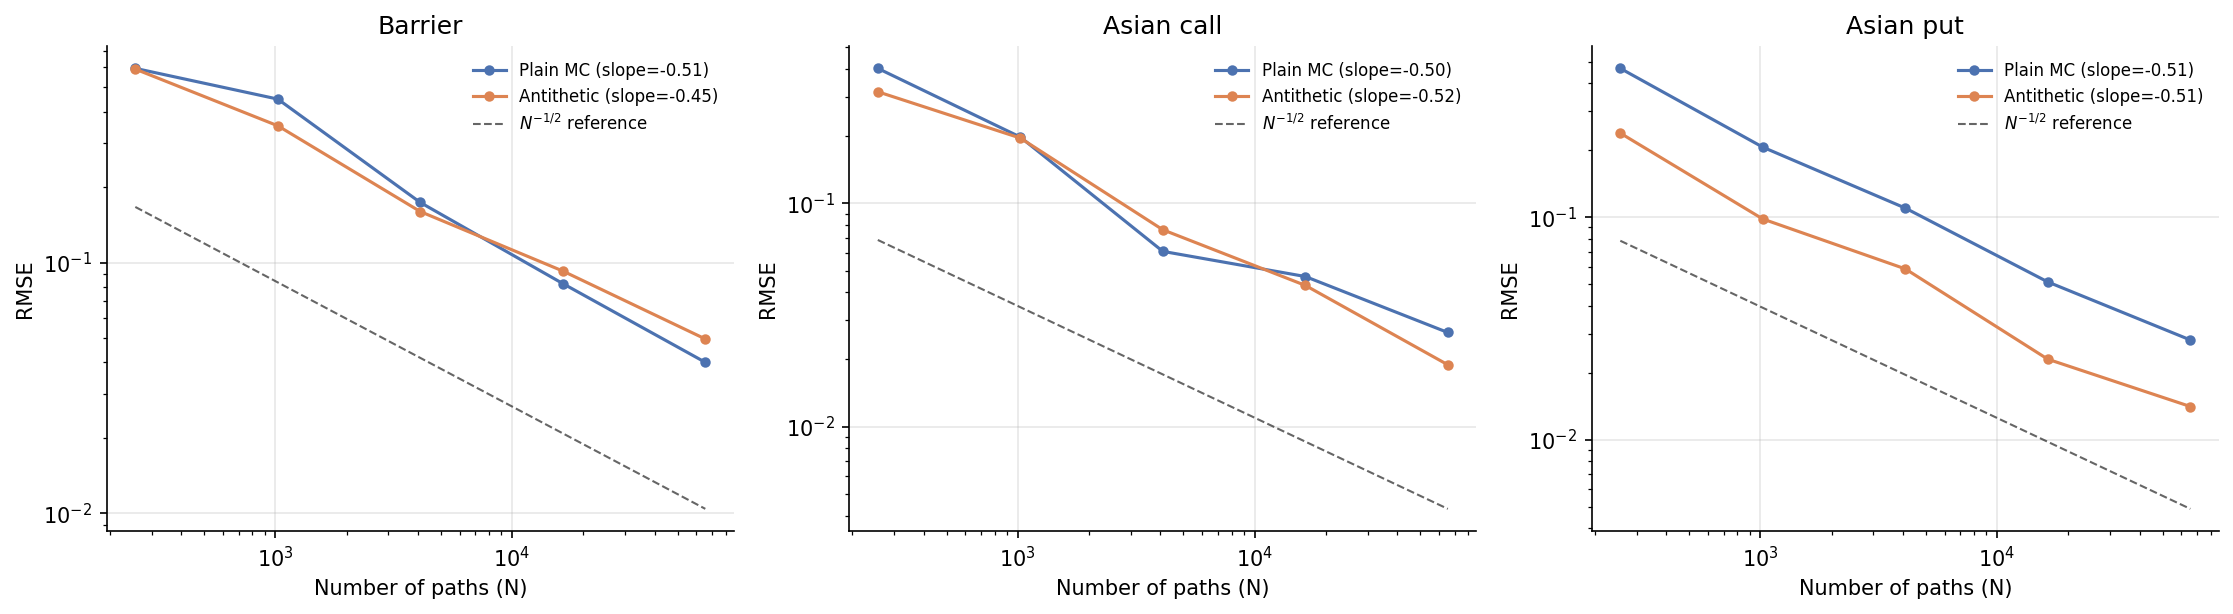
\includegraphics[width=0.85\linewidth]{figures/baseline_rmse_vs_n.png}
  \caption{RMSE vs.\ $N$ on log-log axes for the baseline scenarios, with
  fitted slopes close to the theoretical $N^{-1/2}$ rate.}
  \label{fig:baseline-rmse}
  \Description{A log-log plot of root-mean-squared error against the number
  of simulated paths, with straight declining lines whose slopes are close
  to minus one half.}
\end{figure*}

\paragraph{Sensitivity to the averaging window} The base paper also prices a
geometric Asian call averaged over the last 30 days. Its discrete closed
form is the same formula with a different averaging grid, and the price is
highly sensitive to that grid: $6.708$ for a 30-date window against $3.000$
for the full 252-date window (vanilla call: $7.128$). Our antithetic
estimate at $N=65{,}536$, $6.698\pm0.0066$, validates the 30-date value. The
mechanism is that a shorter window averages over less of the path, so the
volatility of the average approaches that of $S_T$ and the price moves
toward the vanilla call; reading ``30 days'' as about 21 trading days gives
$\approx6.84$, closer still. The antithetic gain changes only modestly
($1.48\times$ vs.\ $1.35\times$, both predicted by $1/(1+\rho)$), so the
window affects the price far more than it affects the sampling method.

\paragraph{The discrete-monitoring bias} Our initial estimate of the 252-step discretely monitored barrier price was $\approx 7.076$ (bias
$\approx -0.03$). A high-precision in-out-parity computation (SE $0.0002$)
instead gives $\mathbf{7.0941}$, a bias of only $\mathbf{-0.0114}$ against
the continuous formula, confirmed independently by the control-variate
estimator (Section~\ref{sec:results-cv}) and by the 64-scramble RQMC
reference (Table~\ref{tab:refs}). At $N=1{,}024$, a single plain-MC run's
standard error ($\approx 0.39$) is about $34\times$ larger than this bias,
so plain Monte Carlo cannot see it at any practical sample size. The bias
grows sharply with the barrier level: on the deep barrier it is $-0.160$
($4.5\%$ of the price), $14\times$ the paper barrier's. Only paths that
cross $B$ and then finish below it can be affected by a missed crossing,
since a path finishing above $B$ is caught on the last date; that exposed
part is $33\%$ of the deep barrier's continuous value but only $3\%$ of the
paper barrier's. The BGK correction over-corrects both, landing about 8 SE
below the deep-barrier reference. Any deep-barrier RMSE taken against the
continuous formula would be dominated by this $0.16$ bias, which exceeds
the error of every variance-reduced method; this is why every RMSE in this
report is measured against the 252-date references.

\subsection{Control Variates: Arithmetic Asian and the Barrier Collapse}
\label{sec:results-cv}
At $N=65{,}536$, the control-variate estimate of the arithmetic Asian call is
$3.162776\pm 0.000361$ (95\% CI of the replicated mean), with correlation
$\rho=0.999488$ against its geometric-Asian control and an observed
within-run variance-reduction factor of $975.7\times$, matching the
theoretical $1/(1-\rho^2)=976.6\times$ almost exactly. An independent
2{,}000{,}000-path plain-MC run gives $3.162517\pm0.008511$, within 0.06
combined standard errors --- validating the arithmetic-Asian price without a
closed form to check against. Figure~\ref{fig:cv-asian} shows the observed
VRF tracking the theoretical value at every $N$, and
Figure~\ref{fig:cv-rho-vrf} confirms the $1/(1-\rho^2)$
relationship across every scenario and sample size tested.

\begin{figure}[t]
  \centering
  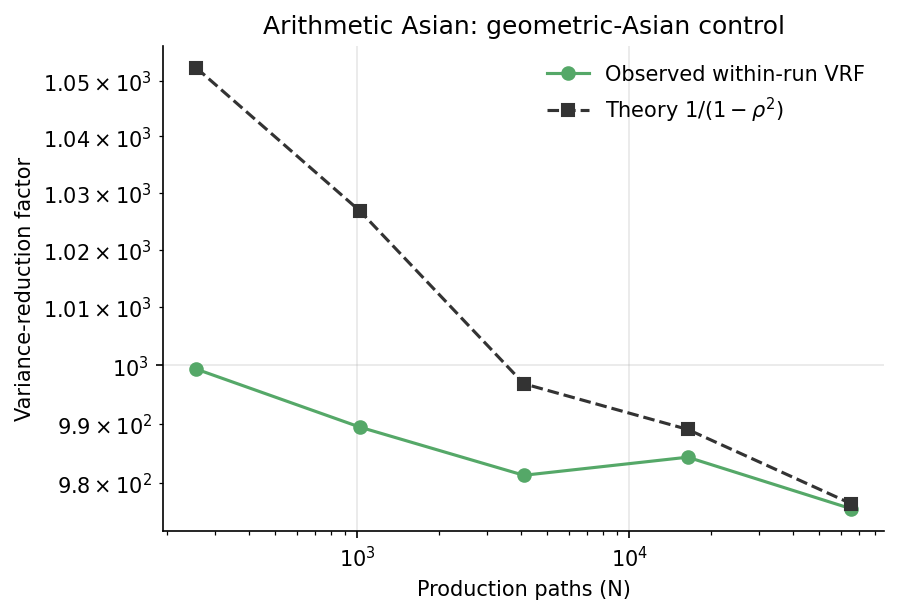
\includegraphics[width=\linewidth]{figures/cv_asian_vrf.png}
  \caption{Control-variate variance-reduction factor for the arithmetic
  Asian call: observed vs.\ theoretical $1/(1-\rho^2)$, stable at
  $\approx 10^3$ across the sample grid.}
  \label{fig:cv-asian}
  \Description{A plot comparing the observed and theoretically predicted
  variance reduction factor of the control variate estimator across sample
  sizes, with the two curves nearly overlapping around one thousand.}
\end{figure}

\begin{figure}[t]
  \centering
  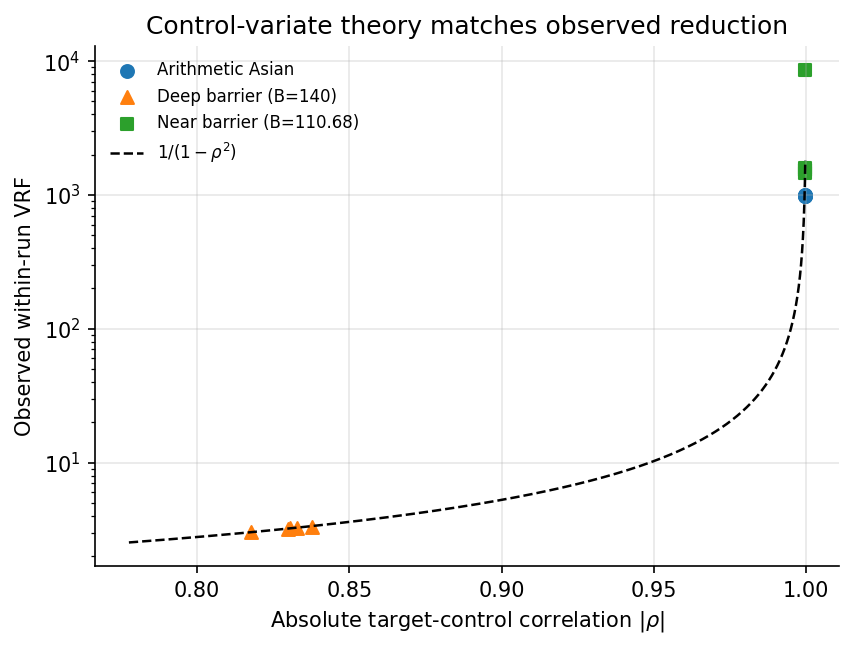
\includegraphics[width=\linewidth]{figures/cv_rho_vs_vrf.png}
  \caption{Observed variance-reduction factor vs.\ correlation $\rho$,
  compared with the theoretical curve $1/(1-\rho^2)$, across all tested
  scenarios.}
  \label{fig:cv-rho-vrf}
  \Description{A scatter plot of variance reduction factor against
  correlation, following a curve that rises sharply as correlation
  approaches one, matching the theoretical prediction closely.}
\end{figure}

The same control (a terminal European call) behaves very differently on two
barriers. On the paper barrier ($B=110.68$), where the up-and-out leg is
worth only about 0.3\% of the price, the up-and-in payoff is almost
identical to a vanilla call path by path, giving $\rho=0.9997$ and a VRF of
$\mathbf{1542\times}$. On the deep barrier ($B=140$), many in-the-money
vanilla-call paths never knock in, so the correlation collapses to
$\rho=0.830$ and the VRF falls to only $\mathbf{3.2\times}$
(Figure~\ref{fig:cv-collapse}). This is the central pedagogical result of
this technique: a control variate's value is not intrinsic, but depends
entirely on how closely it tracks the specific target.

\begin{figure}[t]
  \centering
  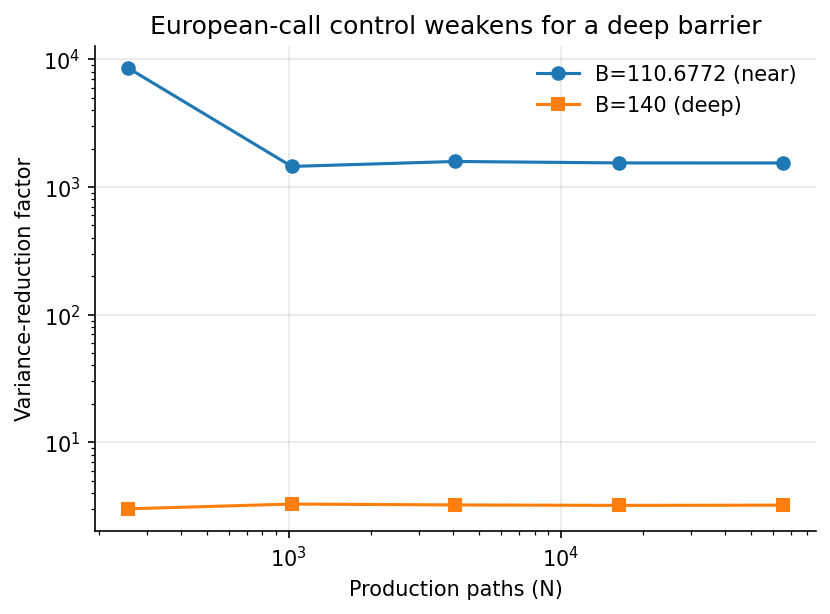
\includegraphics[width=\linewidth]{figures/cv_barrier_collapse.png}
  \caption{The vanilla-call control variate on the paper barrier
  (near-perfect, VRF $\approx 1542\times$) versus the deep barrier (weak,
  VRF $\approx 3.2\times$).}
  \label{fig:cv-collapse}
  \Description{A comparison plot showing the control variate working very
  well for one barrier level and performing only marginally better than
  plain Monte Carlo for a barrier further from the current price.}
\end{figure}

The same estimator, applied with 12, 52, and 252 monitoring dates, resolves
the discrete-monitoring bias directly: at 252 dates it measures
$-0.011945$, matching Section~\ref{sec:results-baseline}'s reference to
within $0.0006$, and resolves it at $54.1$ standard errors of the replicated mean. The BGK
correction is accurate to within $0.0006$--$0.0011$ at 252 dates but
over-corrects substantially at coarser monitoring
(Figure~\ref{fig:barrier-bias}), confirming it is an asymptotic
approximation rather than an exact discrete-barrier formula.

\begin{figure}[t]
  \centering
  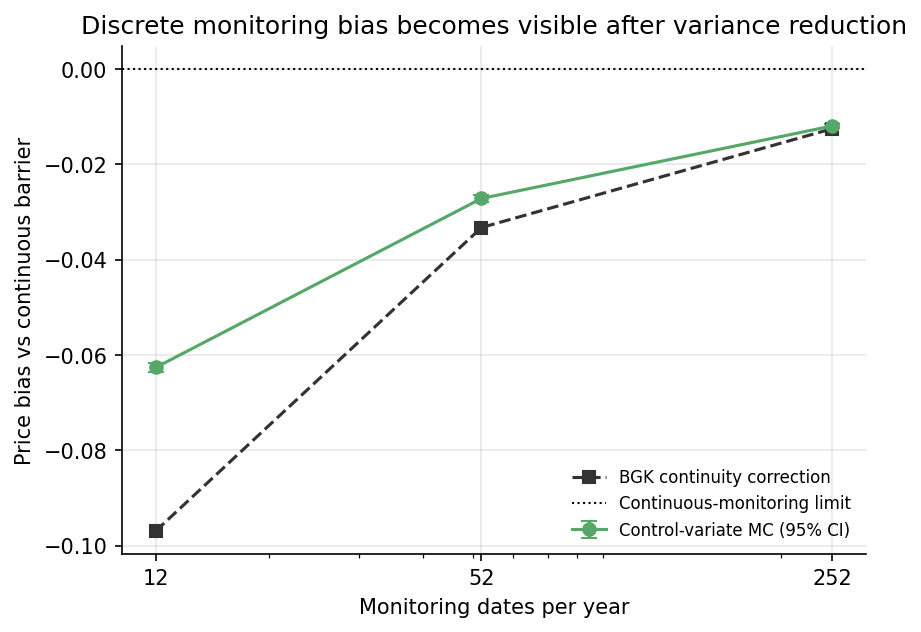
\includegraphics[width=\linewidth]{figures/barrier_bias_vs_steps.png}
  \caption{Discrete-monitoring bias vs.\ number of monitoring dates, measured
  by the control-variate estimator, against the BGK continuity correction.}
  \label{fig:barrier-bias}
  \Description{A plot showing the gap between discretely monitored and
  continuous barrier option prices shrinking as the number of monitoring
  dates increases, with a correction formula tracking it closely at high
  monitoring frequency but overshooting at low frequency.}
\end{figure}

\subsection{Quasi-Monte Carlo Convergence}
\label{sec:results-qmc}
Measured against the 252-date reference, bridge-constructed RQMC achieves
RMSE-vs-$N$ slopes of $-0.80$ on the paper barrier, $-0.60$ on the deep
barrier, and $-0.72$ on the geometric Asian call, all steeper than plain
MC's $\approx -0.5$ (Figures~\ref{fig:qmc-asian} and~\ref{fig:qmc-barrier}). Measuring the paper
barrier against the \emph{continuous} formula instead would have given a
misleadingly flat slope of $-0.26$, since the $-0.011$ monitoring bias would
floor the apparent error once RQMC's own error dropped below it --- a direct
illustration of why the reference price must match the simulation's
monitoring frequency. At $N=65{,}536$ in this experiment's own run, RQMC's
variance-reduction factor reaches $6988\times$ on the paper barrier,
$1052\times$ on the geometric Asian, and $45.5\times$ on the deep barrier
(the independent master sweep of Section~\ref{sec:results-master} gives
$5723\times$ and $40\times$ on the two barriers, well within their
$F$-distribution confidence intervals); the barrier's large gain mirrors
the control variate's $1542\times$ for the same reason, that the option is
nearly a one-dimensional function of the terminal price. The Brownian bridge
construction is responsible for nearly all of this gain: it concentrates
$100\%$ of $\mathrm{Var}(\log S_T)$ and $75$--$98\%$ of
$\mathrm{Var}(\log G)$ (the Asian average) into the first few Sobol
dimensions, where the sequence is most uniform
(Figure~\ref{fig:qmc-effdim}), giving a further $27$--$536\times$ reduction
in variance over the naive incremental construction
(Figure~\ref{fig:qmc-bridge}). Table~\ref{tab:qmc-slopes} gives every slope
with its bootstrap 95\% CI; every plain-MC slope is consistent with $-0.5$.

\begin{table}[t]
\caption{RMSE-vs-$N$ slopes against the 252-date references, with 2{,}000-resample
bootstrap 95\% CIs (QMC experiment, $R=20$).}
\label{tab:qmc-slopes}
\small
\begin{tabular}{lccc}
\toprule
\textbf{Scenario} & \textbf{Plain MC} & \textbf{RQMC, bridge} & \textbf{RQMC, incremental} \\
\midrule
Geometric Asian & $-0.57$ & $\mathbf{-0.72}$ {\scriptsize[$-0.78,-0.65$]} & $-0.61$ \\
Paper barrier & $-0.52$ & $\mathbf{-0.80}$ {\scriptsize[$-0.88,-0.71$]} & $-0.76$ \\
Deep barrier & $-0.44$ & $\mathbf{-0.60}$ {\scriptsize[$-0.67,-0.52$]} & $-0.58$ \\
\bottomrule
\end{tabular}
\end{table}

\begin{figure*}[t]
  \centering
  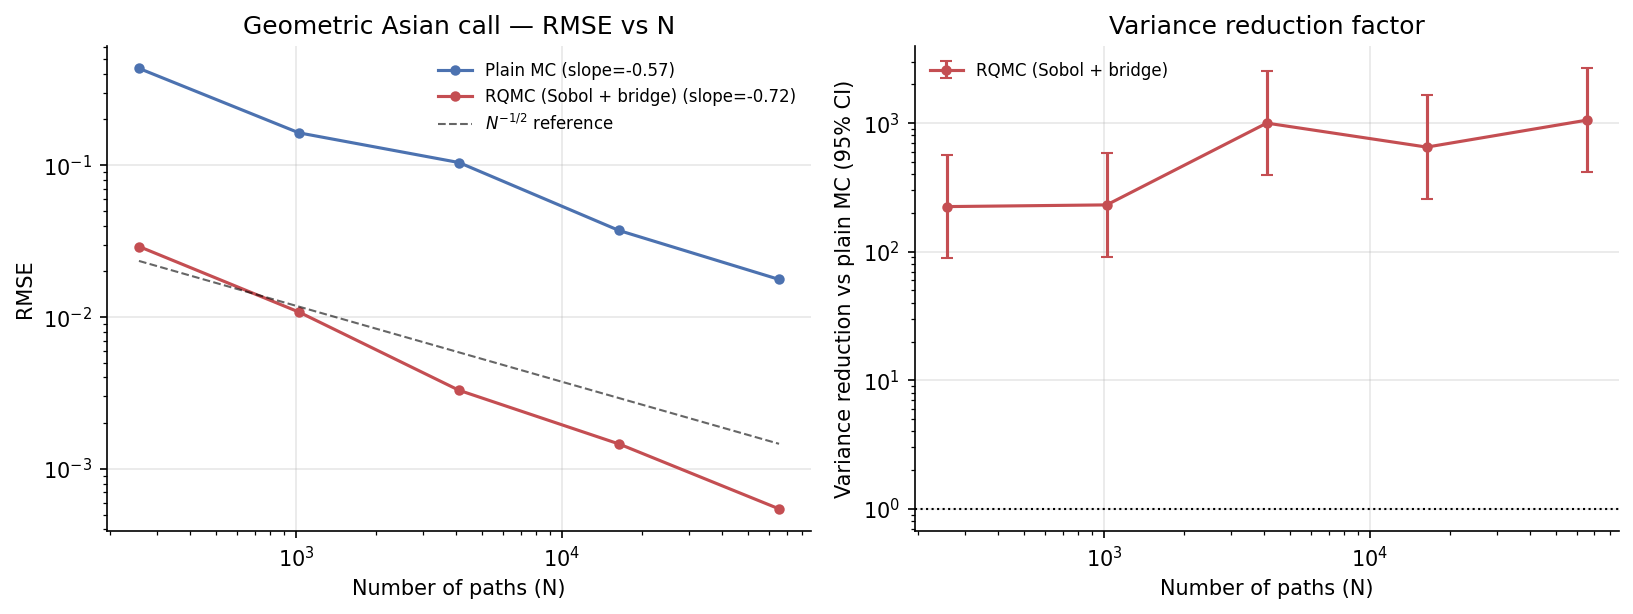
\includegraphics[width=0.85\linewidth]{figures/qmc_vs_mc_asian.png}
  \caption{Geometric Asian call: RMSE vs.\ $N$ for plain MC and RQMC with a
  Brownian bridge (left), and RQMC's variance-reduction factor with
  $F$-distribution 95\% CIs (right).}
  \label{fig:qmc-asian}
  \Description{Left, a log-log plot where the quasi-Monte Carlo error line
  starts lower and falls more steeply than the plain Monte Carlo line.
  Right, the variance reduction factor rising from about two hundred to
  about one thousand as the number of paths grows.}
\end{figure*}

\paragraph{Why the rates differ} We expected RQMC to help barriers less than Asians, because a barrier's payoff is discontinuous. The
mechanism holds, but the grouping does not. The \emph{deep} barrier behaves
as predicted ($-0.60$, VRF $45\times$): its knock-in depends on the path
maximum, a jump spread over many bridge coordinates whose boundary is not
axis-aligned, the same effect the orthant smoke test shows in two
dimensions. The \emph{paper} barrier is the exception ($-0.80$, the largest
gain in the study): at $B=110.68$ the up-and-out leg is worth only $0.023$,
so the payoff is almost exactly $(S_T-K)^+$, and under the bridge $S_T$
depends on Sobol dimension 0 alone. The integrand is effectively
one-dimensional with a single kink, QMC's best case. This contradicted our expectation, so we investigated before reporting it: the
RQMC mean agrees with two independent references, the bridge passes its
orthogonality tests, and the effect matches the control variate's
$1542\times$ on the same option. The \emph{Asian} slope, $-0.72$, falls
short of the predicted $-0.9$: the bridge puts $98.4\%$ of
$\mathrm{Var}(\log G)$ in the first four dimensions, but the remaining
$1.6\%$ is spread thinly over hundreds of poorly balanced high-index
dimensions and decays almost at the MC rate, and the payoff kink slows the
fast part too.

\paragraph{Fixed cost and efficiency} Scrambling a 252-dimensional Sobol
generator costs about 35\,ms per estimate, against 3--4\,ms for an entire
plain-MC run at $N=256$. At $N=256$ on the deep barrier RQMC is therefore
\emph{less} efficient than plain MC ($0.4\times$ here, $0.45\times$ in the
master sweep), and it pays off only from
$N\approx1{,}024$. Because its error also falls faster, its advantage grows
with $N$: at $N=65{,}536$ the bootstrap efficiency ratios in this run are
$621$ [$303$, $1372$] (geometric Asian), $3768$ [$1729$, $8954$] (paper
barrier) and $24.7$ [$8.6$, $62.3$] (deep barrier), with RQMC costing
$1.7$--$1.85\times$ plain MC per estimate (timings indicative; the master
sweep is authoritative).

\paragraph{Validation} Since RQMC has no per-run CI, each cell is checked with
a $t$-interval over its 20 scrambles: all 45 cells of all three methods lie
within 3 SE of the reference, and the 95\% $t$-interval covers it in 43 of
45 cells.

\begin{figure}[t]
  \centering
  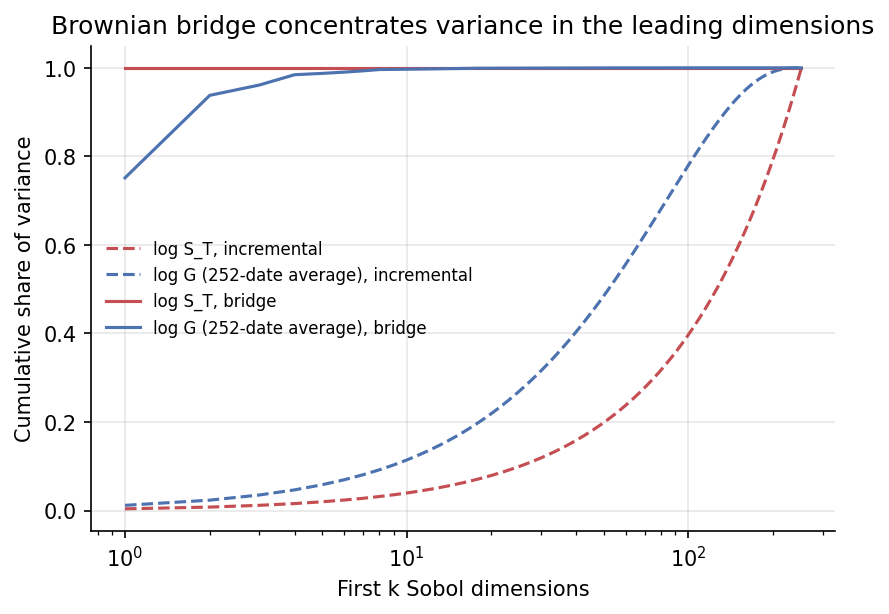
\includegraphics[width=\linewidth]{figures/qmc_effective_dimension.png}
  \caption{Share of the variance of $\log S_T$ and of the log geometric
  average carried by the first $k$ Sobol dimensions, under the Brownian
  bridge (solid) and the incremental construction (dashed). Exact
  calculation from the construction matrix, not a simulation.}
  \label{fig:qmc-effdim}
  \Description{A plot of cumulative variance share against the number of
  leading Sobol dimensions. With the Brownian bridge the terminal price is
  fully determined by the first dimension and the average price is 75
  percent determined by it; with the day-by-day construction both curves
  rise slowly across most of the 252 dimensions.}
\end{figure}

\begin{figure*}[t]
  \centering
  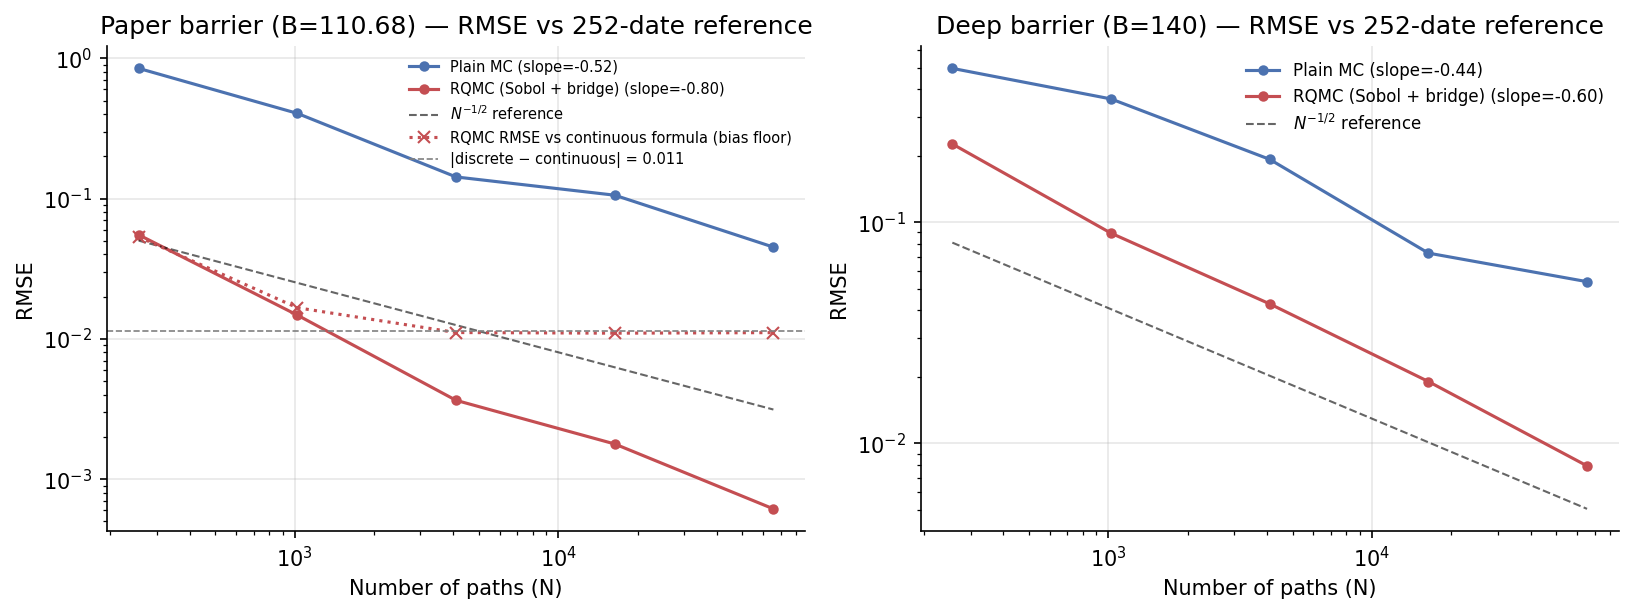
\includegraphics[width=0.85\linewidth]{figures/qmc_vs_mc_barrier.png}
  \caption{RQMC versus plain Monte Carlo on the paper and deep barriers,
  RMSE measured against the 252-date reference.}
  \label{fig:qmc-barrier}
  \Description{A log-log plot comparing the error of randomized
  quasi-Monte Carlo and plain Monte Carlo for two barrier option scenarios,
  with the quasi-Monte Carlo line falling much faster for the easier
  scenario and only modestly faster for the harder one.}
\end{figure*}

\begin{figure*}[t]
  \centering
  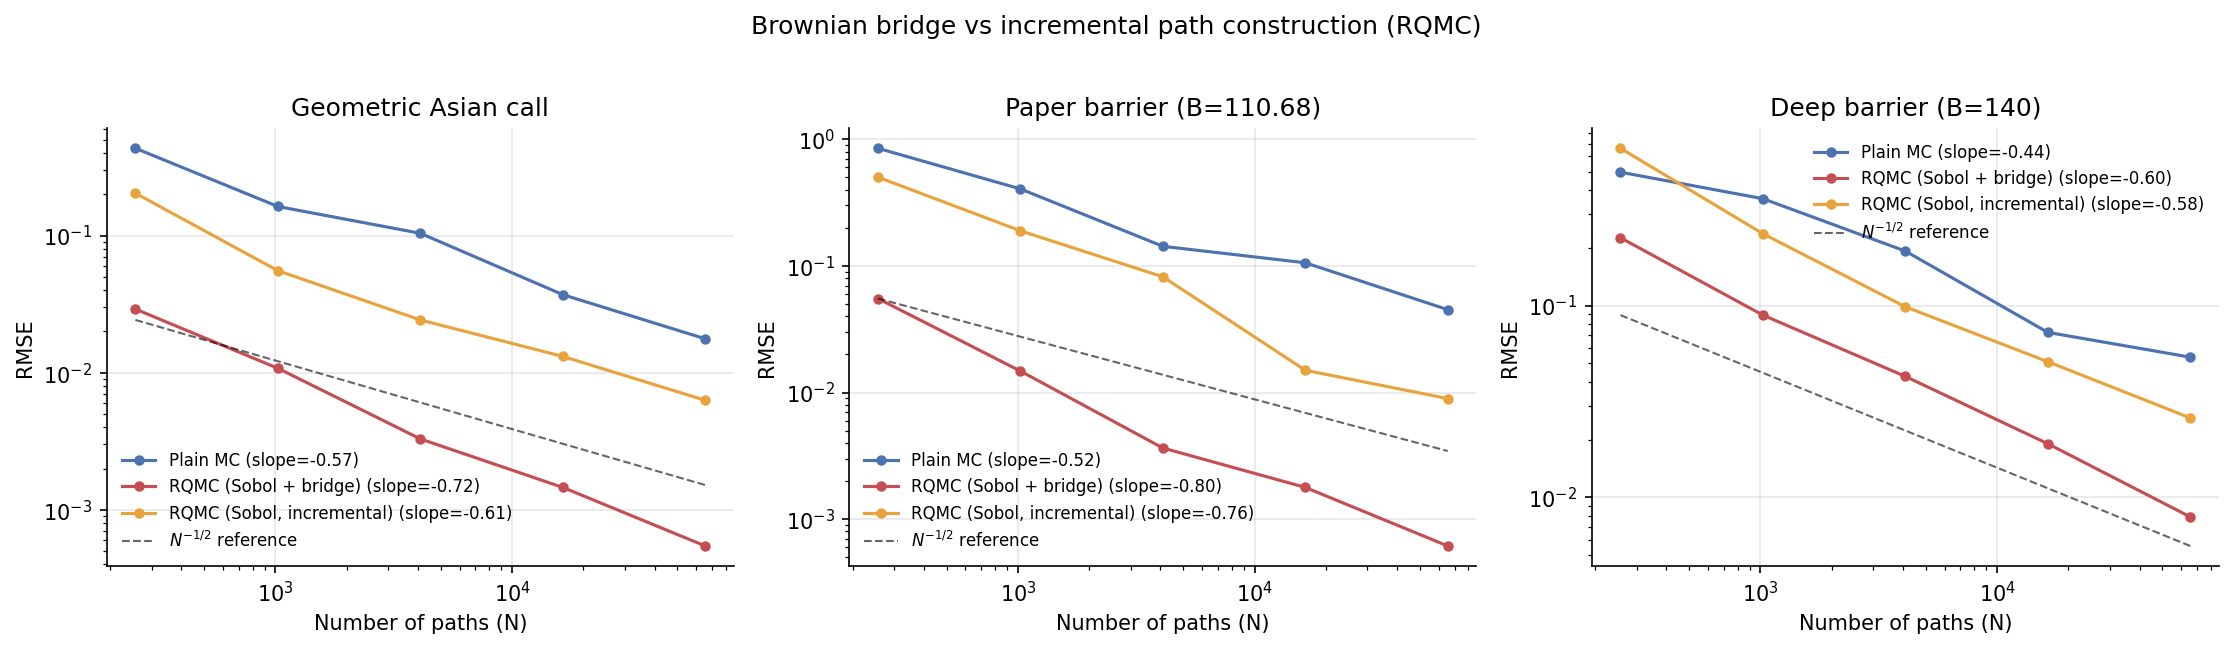
\includegraphics[width=0.85\linewidth]{figures/qmc_bridge_vs_incremental.png}
  \caption{Brownian-bridge versus incremental Sobol-dimension construction,
  across the geometric Asian call, the paper barrier, and the deep barrier.}
  \label{fig:qmc-bridge}
  \Description{A comparison plot showing that assigning the best-quality
  low-discrepancy dimensions to the overall shape of the price path, rather
  than to individual days in sequence, substantially reduces estimator
  variance across all three option scenarios tested.}
\end{figure*}

\subsection{Importance Sampling for Rare Barrier Crossings}
\label{sec:results-is}
Table~\ref{tab:is-headline} summarizes importance sampling at
$N=65{,}536$ on three barriers of increasing rarity: the paper barrier
(60\% knock-in probability), the deep barrier (9.3\%), and the extension
scenario \texttt{rare\_barrier} at $B=160$ (1.9\%).

\begin{table}[t]
\caption{Importance sampling at $N=65{,}536$: within-run variance-reduction
factor and efficiency vs.\ plain MC. Paper and deep barriers: master sweep;
rare barrier: the importance-sampling experiment (indicative timing).}
\label{tab:is-headline}
\small
\begin{tabular}{lccc}
\toprule
\textbf{Barrier} & \textbf{Knock-in \%} & \textbf{VRF} & \textbf{Efficiency} \\
\midrule
Paper ($B=110.68$) & 60\% & $4.6\times$ & $2.8\times$ \\
Deep ($B=140$) & 9.3\% & $9.8\times$ & $8.6\times$ \\
Rare ($B=160$, extension) & 1.9\% & $22.2\times$ & $\approx 49\times$ \\
\bottomrule
\end{tabular}
\end{table}

The pattern matches theory exactly: importance sampling's advantage grows
as the target event becomes rarer. Figure~\ref{fig:is-deep-barrier} shows
the deep-barrier price converging correctly alongside its efficiency gain
over plain MC across the sample grid; the gain is only visible from
$N\approx 2{,}000$--$4{,}000$ upward, since the 10,000-path pilot's fixed cost
dominates at smaller $N$. Figure~\ref{fig:is-weights} shows the
likelihood-ratio weight distribution at the tuned drift for all three
barriers: although the rare barrier's effective sample size is only $1.1\%$
of $N$, the largest weights fall almost entirely on paths with zero payoff,
so the price estimate is not dominated by a handful of paths --- the top
$1\%$ of paths carry only $6\%$ of the price even in that case.

\begin{figure*}[t]
  \centering
  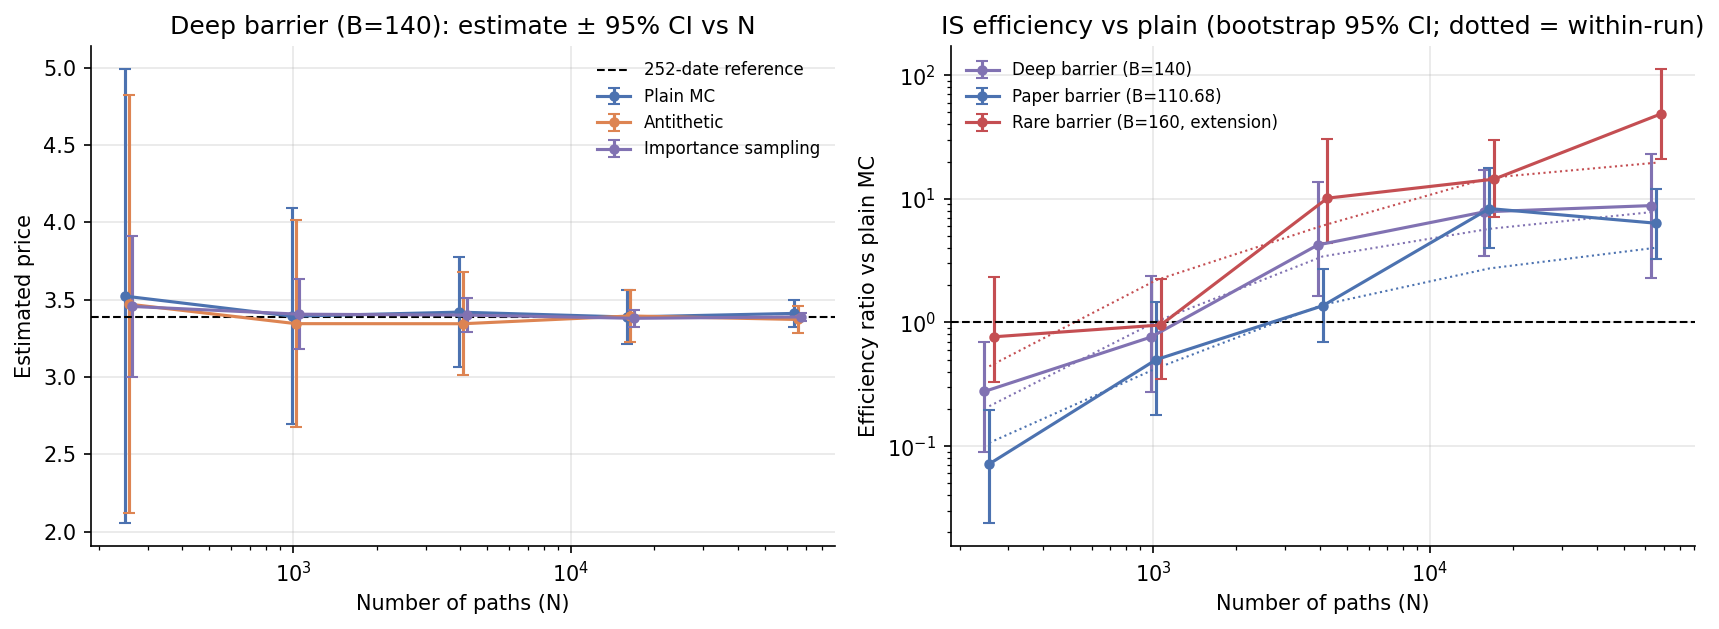
\includegraphics[width=0.85\linewidth]{figures/is_deep_barrier.png}
  \caption{Importance sampling on the deep barrier: price convergence
  (left) and efficiency vs.\ plain MC (right) across the sample grid.}
  \label{fig:is-deep-barrier}
  \Description{Two side-by-side plots: one showing the importance-sampling
  price estimate converging to the reference value with narrowing
  confidence intervals, the other showing its efficiency advantage over
  plain Monte Carlo growing with sample size after an initial region where
  it is less efficient.}
\end{figure*}

\begin{figure*}[t]
  \centering
  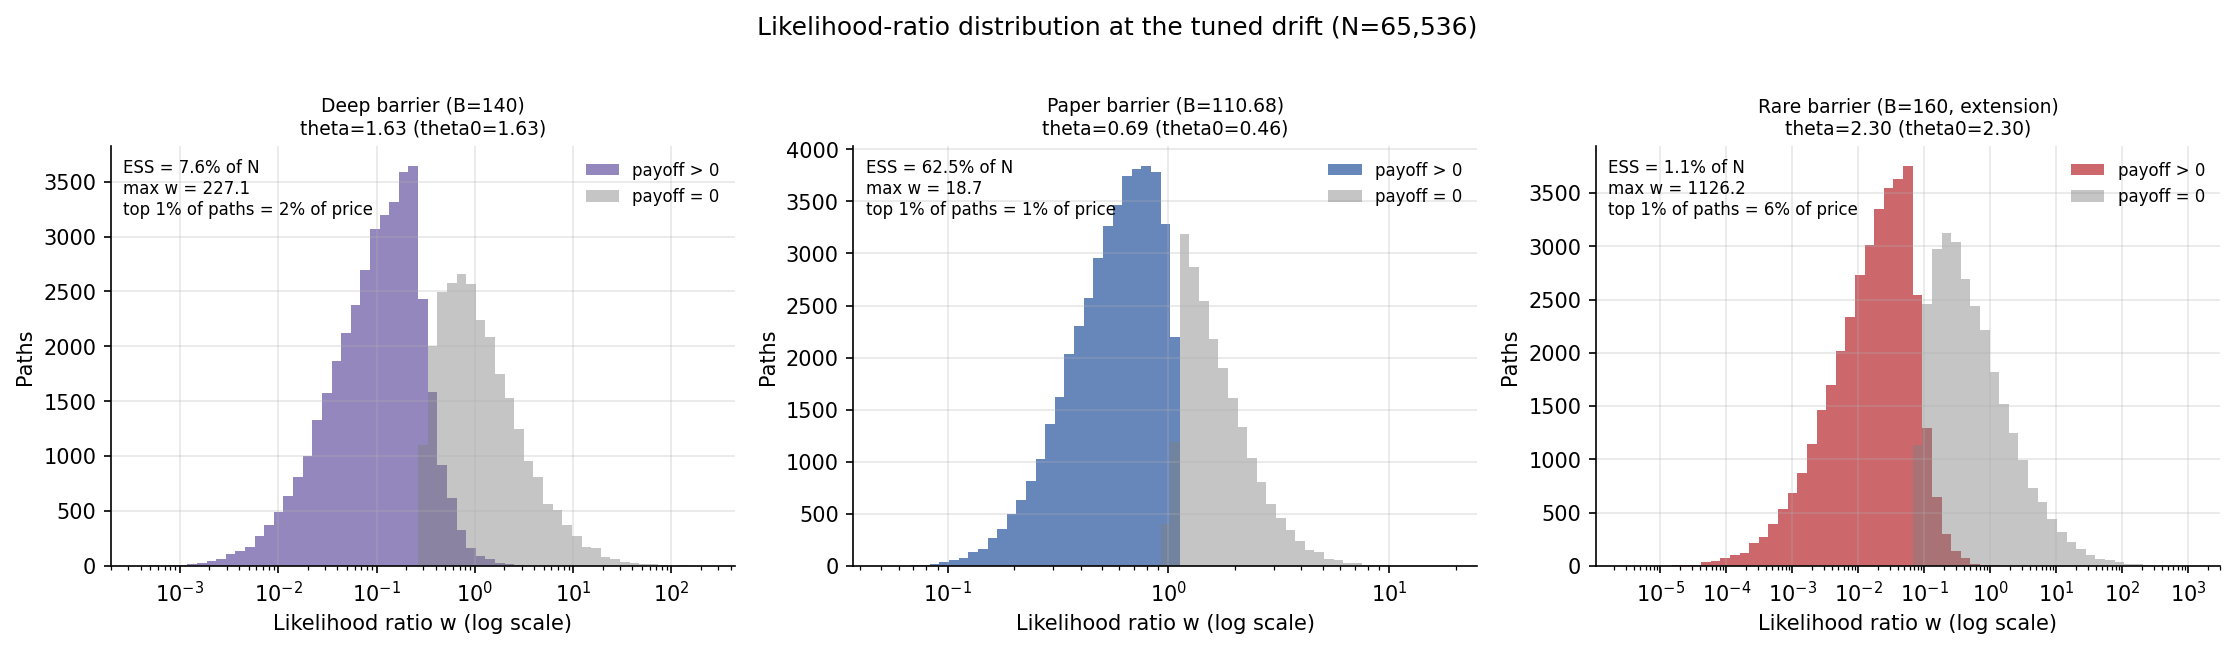
\includegraphics[width=0.85\linewidth]{figures/is_weight_distribution.png}
  \caption{Likelihood-ratio weight distributions at the tuned drift, for the
  deep barrier, the paper barrier, and the rare extension barrier.}
  \label{fig:is-weights}
  \Description{Three histograms of simulation path weights on a logarithmic
  scale, showing that paths with zero payoff carry most of the largest
  weights across all three barrier levels, while the effective sample size
  shrinks as the barrier level moves further from the current price.}
\end{figure*}

\subsection{Master Comparison of All Five Methods}
\label{sec:results-master}
Table~\ref{tab:master} gives the headline result of the project: efficiency
relative to plain Monte Carlo at $N=65{,}536$, from the single authoritative,
interleaved run (Section~\ref{sec:master-protocol}), with bootstrap 95\%
confidence intervals.

\begin{table*}[t]
\caption{Master comparison: efficiency relative to plain Monte Carlo at $N=65{,}536$, with 95\% bootstrap confidence intervals. ``n/a'' marks a method not applicable to that option.}
\label{tab:master}
\small
\begin{tabular}{lcccc}
\toprule
\textbf{Method} & \textbf{Paper barrier} & \textbf{Deep barrier} & \textbf{Arithmetic Asian} & \textbf{Geometric Asian} \\
\midrule
Plain MC & $1$ & $1$ & $1$ & $1$ \\
Antithetic & $1.2$ [$0.5$, $2.8$] & $1.1$ [$0.5$, $2.9$] & $0.97$ [$0.35$, $2.6$] & $1.1$ [$0.5$, $2.9$] \\
Control variate & $1{,}602$ [$656$, $4{,}276$] & $4.2$ [$1.6$, $10.0$] & $770$ [$266$, $1{,}970$] & n/a \\
\textbf{RQMC + bridge} & $\mathbf{2{,}260}$ [$1{,}065$, $5{,}050$] & $\mathbf{21.3}$ [$7.9$, $51.4$] & $\mathbf{794}$ [$269$, $2{,}120$] & $\mathbf{791}$ [$358$, $1{,}638$] \\
Importance sampling & $2.8$ [$1.3$, $5.7$] & $8.6$ [$3.0$, $37.8$] & n/a & n/a \\
\bottomrule
\end{tabular}
\end{table*}

Figure~\ref{fig:master-bars} shows the same comparison graphically, and
Figure~\ref{fig:master-rmse} shows the RMSE-vs-$N$ curves for every method on
every scenario, from which the headline efficiency numbers are derived.

\begin{figure*}[t]
  \centering
  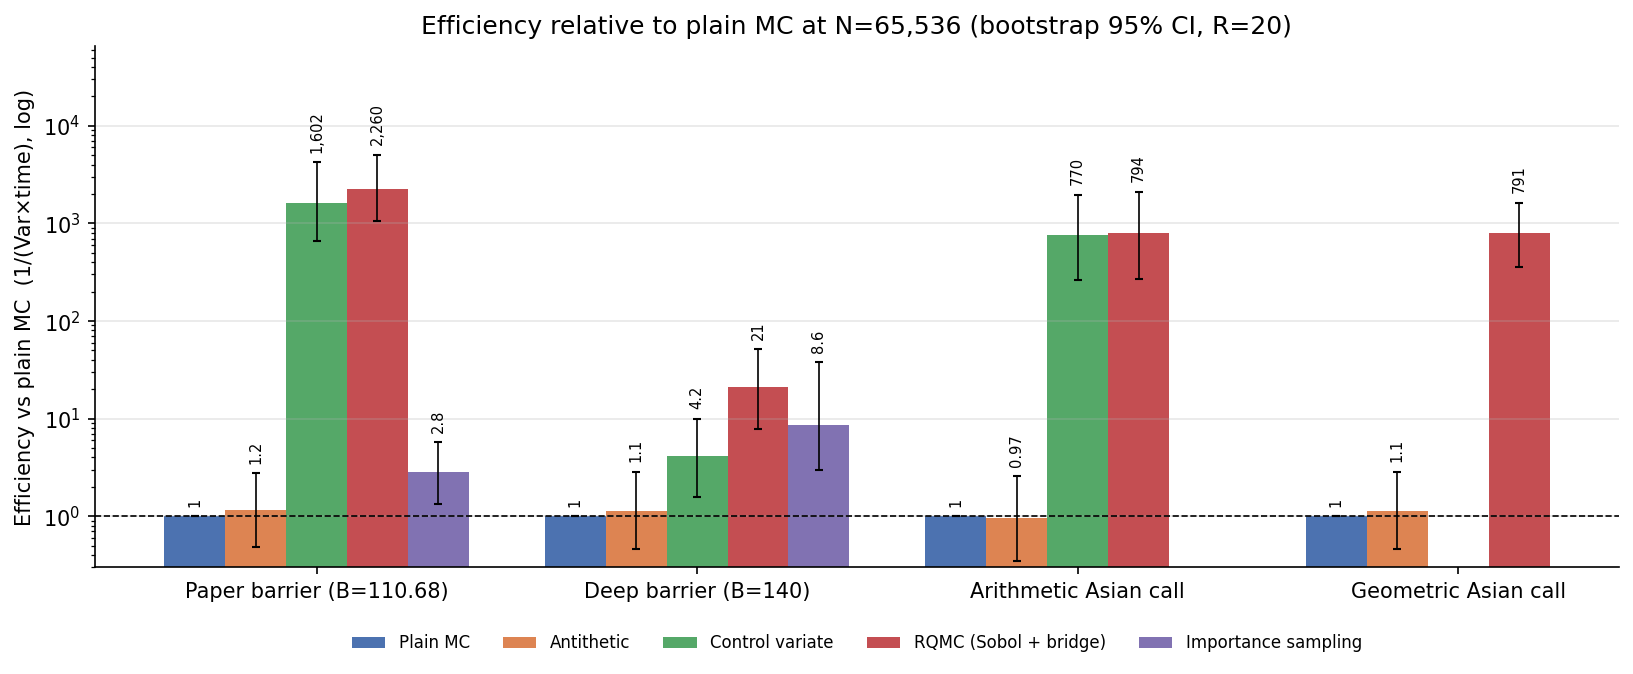
\includegraphics[width=0.85\linewidth]{figures/master_efficiency_bars.png}
  \caption{Efficiency vs.\ plain Monte Carlo across all five methods and all
  four scenarios, at $N=65{,}536$ (log scale).}
  \label{fig:master-bars}
  \Description{A grouped bar chart on a logarithmic scale comparing five
  pricing methods across four option scenarios, showing control variates
  and randomized quasi-Monte Carlo far ahead of the others on three of the
  four scenarios, with randomized quasi-Monte Carlo also leading on the
  hardest scenario and importance sampling second there.}
\end{figure*}

\begin{figure*}[t]
  \centering
  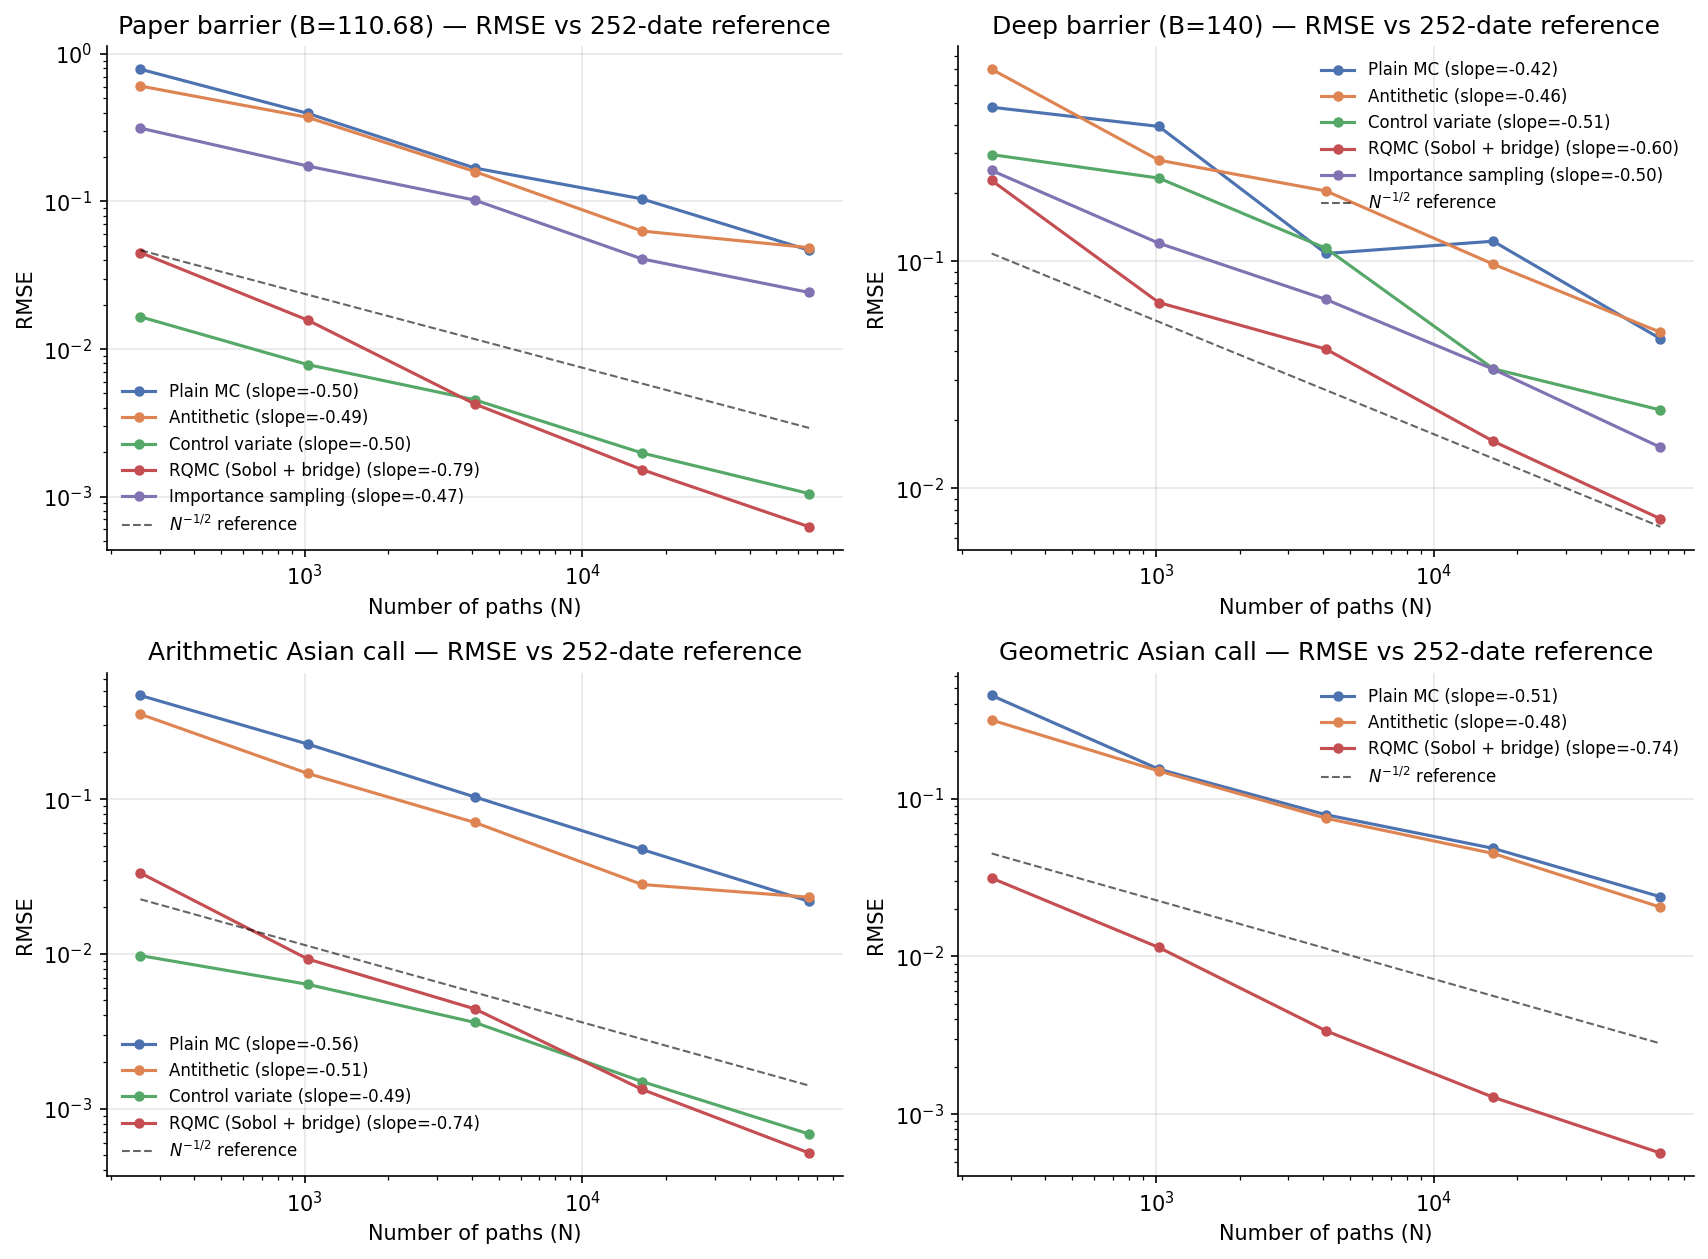
\includegraphics[width=0.85\linewidth]{figures/master_rmse_vs_n.png}
  \caption{RMSE vs.\ $N$ for every method on every scenario, from the master
  sweep (log-log axes).}
  \label{fig:master-rmse}
  \Description{A grid of four log-log plots, one per option scenario, each
  showing the error-versus-sample-size curves for every pricing method,
  with the quasi-Monte Carlo method's curve falling at a visibly steeper
  slope than the others in most panels.}
\end{figure*}

Three findings stand out. First, antithetic variates deliver the gain
measured in Section~\ref{sec:results-baseline} --- within-run variance
ratios of $1.4$--$1.5\times$ on the paper barrier and both Asians at no
extra cost per path --- but a gain of that size is smaller than the
$\pm32\%$ sampling noise of a 20-replicate variance estimate, so the
across-replicate efficiency intervals in Table~\ref{tab:master} all
include $1\times$. The techniques that exploit the payoff's structure
reach two to three orders of magnitude more. Second, the control variate and RQMC are
\emph{statistically tied} on the paper barrier and the arithmetic Asian,
because they exploit the same underlying structure (the payoff is nearly a
function of one Gaussian), while RQMC pulls ahead as $N$ grows because it
improves the convergence \emph{rate} rather than just the constant. Third,
the deep barrier is hard for every technique, since its payoff depends on
the path maximum rather than a single coordinate; importance sampling is
the only technique whose advantage grows as the knock-in becomes rarer still
(Table~\ref{tab:is-headline}).

Converting efficiency into a practical number: reaching one-cent accuracy
($\epsilon=0.01$) on the arithmetic Asian needs about 270{,}000 plain-MC
paths (2.3~s) but only 340 control-variate paths (5~ms), roughly
$500\times$ faster; on the deep barrier at $\epsilon=0.001$, plain MC would
need an extrapolated $6.9\times 10^8$ paths (almost two hours), while RQMC
needs about 30~s.

%% =========================================================================
\section{Conclusion and Future Work}
%% =========================================================================

\subsection{Conclusion}
We rebuilt the base paper's experiment from scratch, validated every
estimator against closed forms, and reproduced its two central findings.
Its antithetic speedups ($1.47\times$ barrier, $1.35\times$ Asian call)
are confirmed as variance ratios and are predicted by the pair correlation through $1/(1+\rho)$, which also explains the larger gain on
the in-the-money Asian put and the smaller gain on rarer barriers. Its
conclusion that the discretization scheme has a negligible effect is
confirmed and explained by weak-order theory: Milstein's much better
pathwise accuracy does not reach the price, where both schemes are first
order and their bias is far below the sampling error. Along the way we
quantified how slowly plain Monte Carlo buys precision (about $10^5$ paths
for $\pm1\%$) and how strongly the Asian price depends on its averaging
window. We then implemented three advanced variance-reduction techniques,
the direction the base paper recommends for future work, and benchmarked
all five methods on one efficiency metric from a single authoritative run. Control variates
and randomized quasi-Monte Carlo are $10^2$--$10^3$ times more efficient than
plain Monte Carlo wherever a payoff is nearly a function of one Gaussian;
importance sampling is the specialist for genuinely rare barrier crossings;
and antithetic variates remain a simple, model-free first step whose
modest $1.1$--$1.5\times$ gain depends on how linear the payoff is. Variance reduction additionally makes a real, systematic
discrete-monitoring bias visible that plain Monte Carlo is too noisy to
detect. \textbf{Our recommendation: to reach a target accuracy on a barrier
option, use randomized quasi-Monte Carlo with a Brownian bridge; on the
arithmetic-average Asian option, use the geometric-Asian control variate.}

\subsection{Limitations}
With $R=20$ replicates, efficiency confidence intervals span a factor of
$3$--$5$, so techniques within about $2\times$ of each other (control
variate vs.\ RQMC on two scenarios; RQMC vs.\ IS on the deep barrier) cannot
be statistically ranked. The authoritative timings come from one machine,
single-threaded; cost \emph{ratios} should transfer across machines, but
absolute numbers will not. Our importance-sampling drift search uses a fixed
7-point grid tied to a heuristic starting point, which under-reaches the true
optimum on the paper barrier by about $2.3\times$. Both the control-variate
and importance-sampling estimators are validated only under the exact GBM
scheme; their biases under Euler--Maruyama or Milstein were not
characterized. Finally, our replication fixes the implementation details
the base paper leaves open (step count, random seed, Asian strike and
averaging grid) at the most plausible values; the findings of
Section~\ref{sec:results-baseline} do not depend on these choices among
the alternatives we tried (e.g.\ a 21-trading-day reading of the 30-day
window).

\subsection{Future Work}
Natural next steps are: (1)~combining techniques, e.g.\ RQMC with a control
variate or with importance sampling, which should dominate on the deep
barrier where each alone gains only $9$--$21\times$; (2)~better
importance-sampling drift tuning via cross-entropy or large-deviations
methods; (3)~multilevel Monte Carlo to address discretization error, the
dual problem to the sampling-error reduction studied here; (4)~richer
models (stochastic volatility, double barriers) and products (Greeks), where
variance reduction matters even more; and (5)~a larger replicate count for
the master sweep, to resolve the near-ties identified above.

\section*{Author Contributions}
The project ran as a five-stage relay, with each member owning one stage end
to end (code, tests, experiments, and the corresponding report content);
Stage~6 (assembly) was shared. Nafis Nahian (2105007) built the simulation
engine, estimators, and benchmarking infrastructure, and ran the baseline
replication. Aritra Debnath (2105010) implemented control variates and the
arithmetic-Asian and barrier-bias experiments. Zaki Rehnoom Unmona (2105016)
implemented quasi-Monte Carlo, the Brownian bridge, and the discretization-order
study. Tamzeed Mahfuz (2105012) implemented importance sampling, the master
comparison, and the final synthesis. Arnob Biswas (2105015) built the
analytic closed-form oracles and the foundational configuration and testing
infrastructure that every later stage imports.

%% =========================================================================
\bibliographystyle{ACM-Reference-Format}
\bibliography{references}

%% =========================================================================
\appendix
\section{Reproducing Every Number}
Every number reported in this paper is generated by the code in the GitHub
repository linked after the title. From a fresh clone:
\begin{verbatim}
pip install -r requirements.txt
pytest tests/ -q                   # 90 tests
python run_all.py --analyze-only   # regenerate every figure
                                    # and table from the committed
                                    # raw data (about 2 minutes)
python run_all.py                  # full re-simulation from
                                    # scratch (about 25 minutes,
                                    # single-threaded)
\end{verbatim}
Every price in the repository is produced by a deterministic random seed
keyed on the scenario, method, sample size, and replicate index, so a
re-simulation reproduces every price exactly on the same library versions.
Timings, and therefore efficiency numbers, depend on the machine; the
authoritative timings are those of the master sweep
(Section~\ref{sec:master-protocol}).

\end{document}
